\chapter{Calibration Methods}\label{chap:calibration}
To simulate qubit-resonator trajectories of a readout, we will have to create a model of our system. Throughout chapter \ref{chap:cQED}-\ref{chap:measurements}, we introduced new theory to describe the system, however, this also come with many parameters, we are still left to determine. Estimating these parameters from the qubit in the Laboratory will be  the focus in this chapter. Throughout the process, we will perform multiple fits and only present the important outcomes in the main text. A list of goodness of fit and fit parameters can be found in Appendix \ref{chap:fit_params}.


% In order to use a qubit and in particular if we want to simulate said qubit, we need to learn the most important parameters. In this section, we will go through the different methods used for calibrating a qubit and the connected resonator in order to have a useful qubit along with the possibilities of simulating the system.


\section{Qubit Calibration}
We will start with a calibration of the Transmon. While we could solve the system by finding the values of $E_C$ and $E_J$, we will instead model the Transmon as a three level system and simulate the charge matrix as $\mel{k}{n}{k} = a + a^\dagger$\footnote{This gives us the right correlation between $\ket{0}\leftrightarrow \ket{1}$ and a close to correct connection from $\ket{1}\leftrightarrow\ket{2}$}. This leaves us to determine the frequency $f_{01}$ and the anharmonicity $\alpha$. Furthermore, in order to perform gates, we will calibrate a Rabi pulse. In addition to these parameters, we will determine the characteristic time for energy decay and dephasing  $T_1$ and $T_2$.

\subsection{Spectroscopy}\label{sec:qubit_spectroscopy}
To control the qubit and to simulate its Hamiltonian, perhaps the most important quantity is the frequency. The frequency is found by doing spectroscopy, where a pulse is sent to the qubit at different frequencies. The qubit is then measured to see if it has changed states. The qubit frequency $f_{01}$ will now be the center of a Lorentzian distribution \cite{hucul_trapped_ion}. Thus we can determine $f_{01}$ by fitting such a curve. This is done in the left panel in figure \ref{fig:qubit_spectroscopy}.

Since the design of the transmon gives a negative anharmonicty, we can extend the qubit spectroscopy, to also look for a transition from $\ket{0}\to \ket{2}$. This can be done either with $f_{02}$ or to stay in the frequency regime, we can instead look for a transition from absorption of two photons. Here the two photon will have frequency $f_{02} / 2$. Or formulating it in terms of the anharmonicity at $f_{01} - \alpha / 2$. A fit with two Lorenzians can be found in the right panel in figure \ref{fig:qubit_spectroscopy}. 
% \begin{margintable}
%     \caption{Goodness of Fit for the spectroscopy and anharmonicity experiments.}
%     \centering
%     \begin{tabular}{r|ll}
%         Experiment      & $\chi^2$      &p-value   \\ \hline
%         Spectroscopy    & $127.3$       & $1.8 \%$   \\
%         Anharmonicity   & $882.1$       & $0.0 \%$   \\
%     \end{tabular}
%     \label{tab:spectroscopy fit}
% \end{margintable}
\begin{figure*}[t]
    \caption{Qubit spectroscopy for the $f_{01}$ transition frequency to the left. On the right is an extended scan where another peak is seen, this is the $f_{02}/2$ where two photons are absorbed to go from $ 0 \to 2$. The fits are Lorentzian for one peak and the sum of two Lorenzian for the two peak spectroscopy. }
    \begin{minipage}{0.50\linewidth}
        \centering
        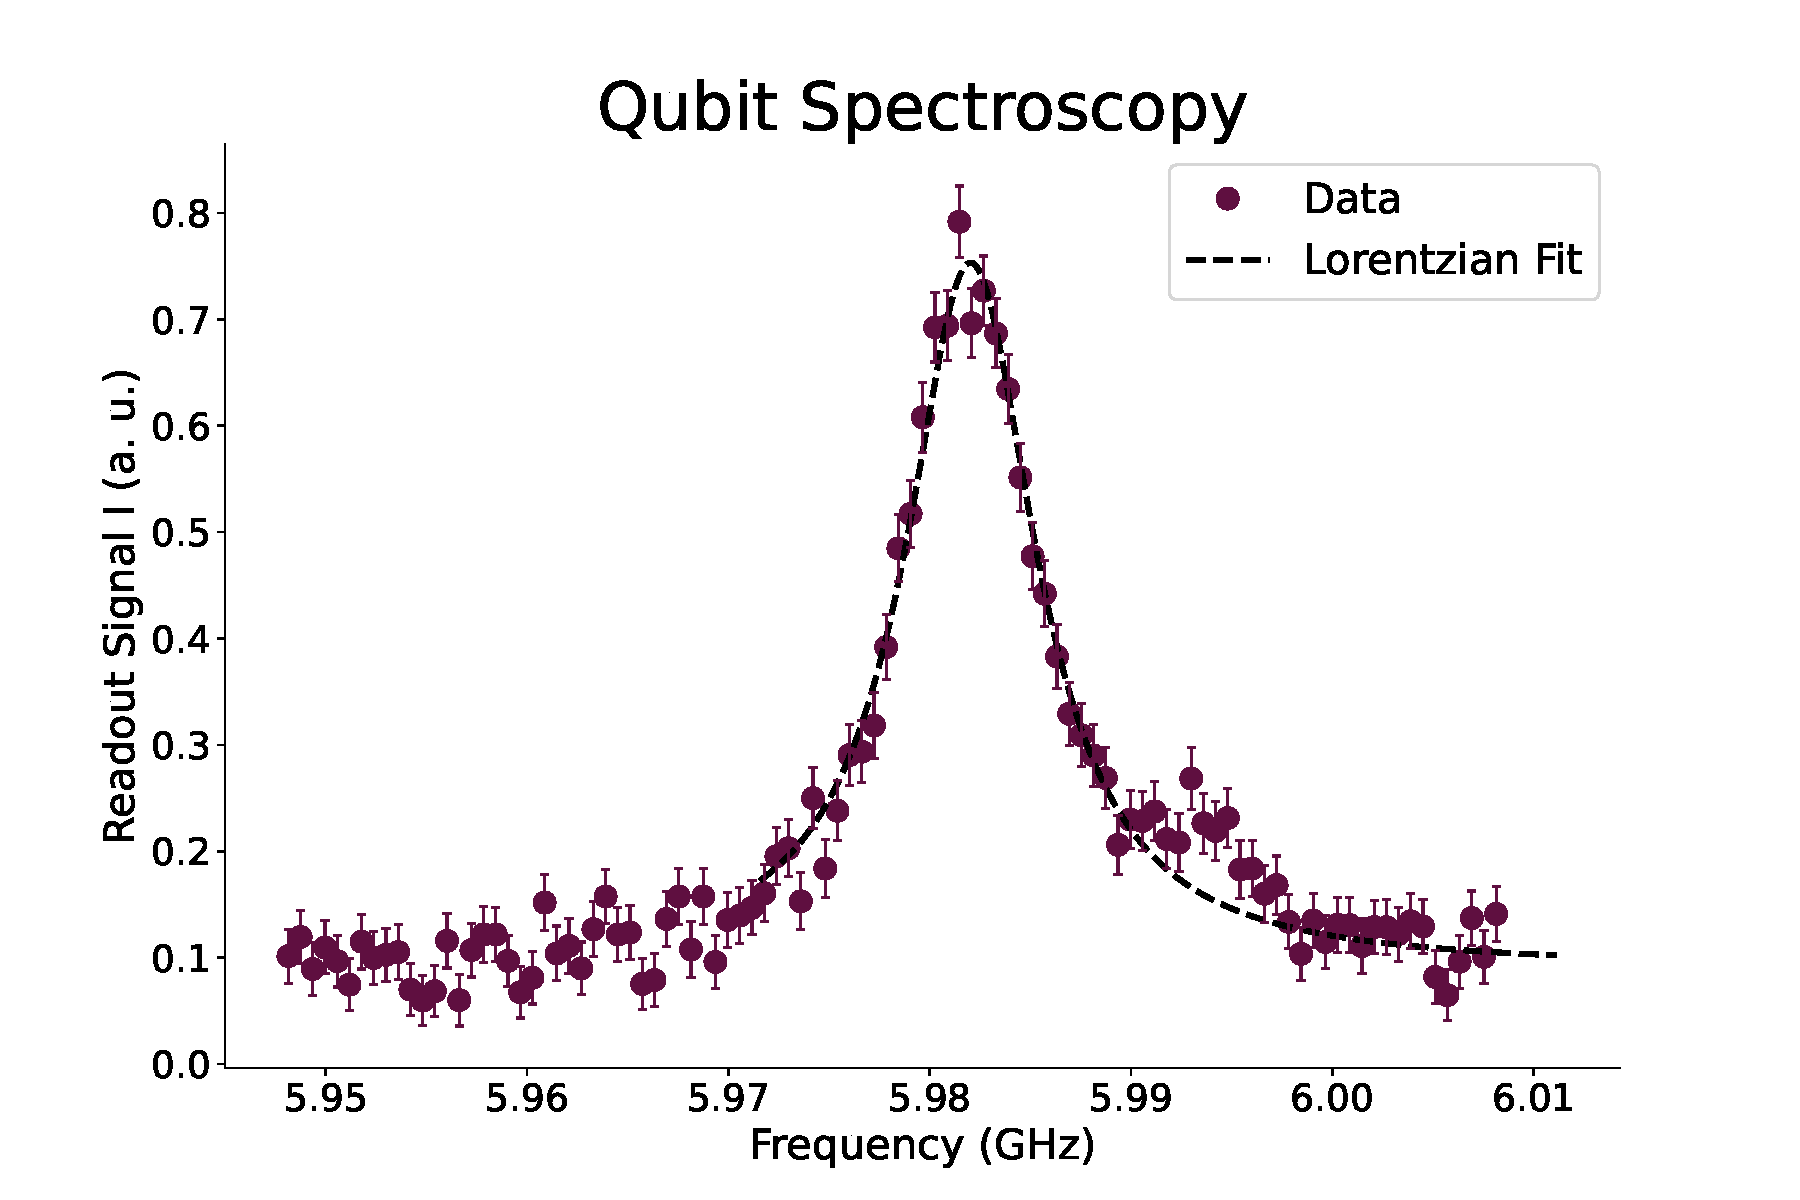
\includegraphics[width=1.0\linewidth]{Calibrations/Figures/Qubit Spectroscopy.pdf} % first figure itself
    \end{minipage}
    \begin{minipage}{0.50\linewidth}
        \centering
        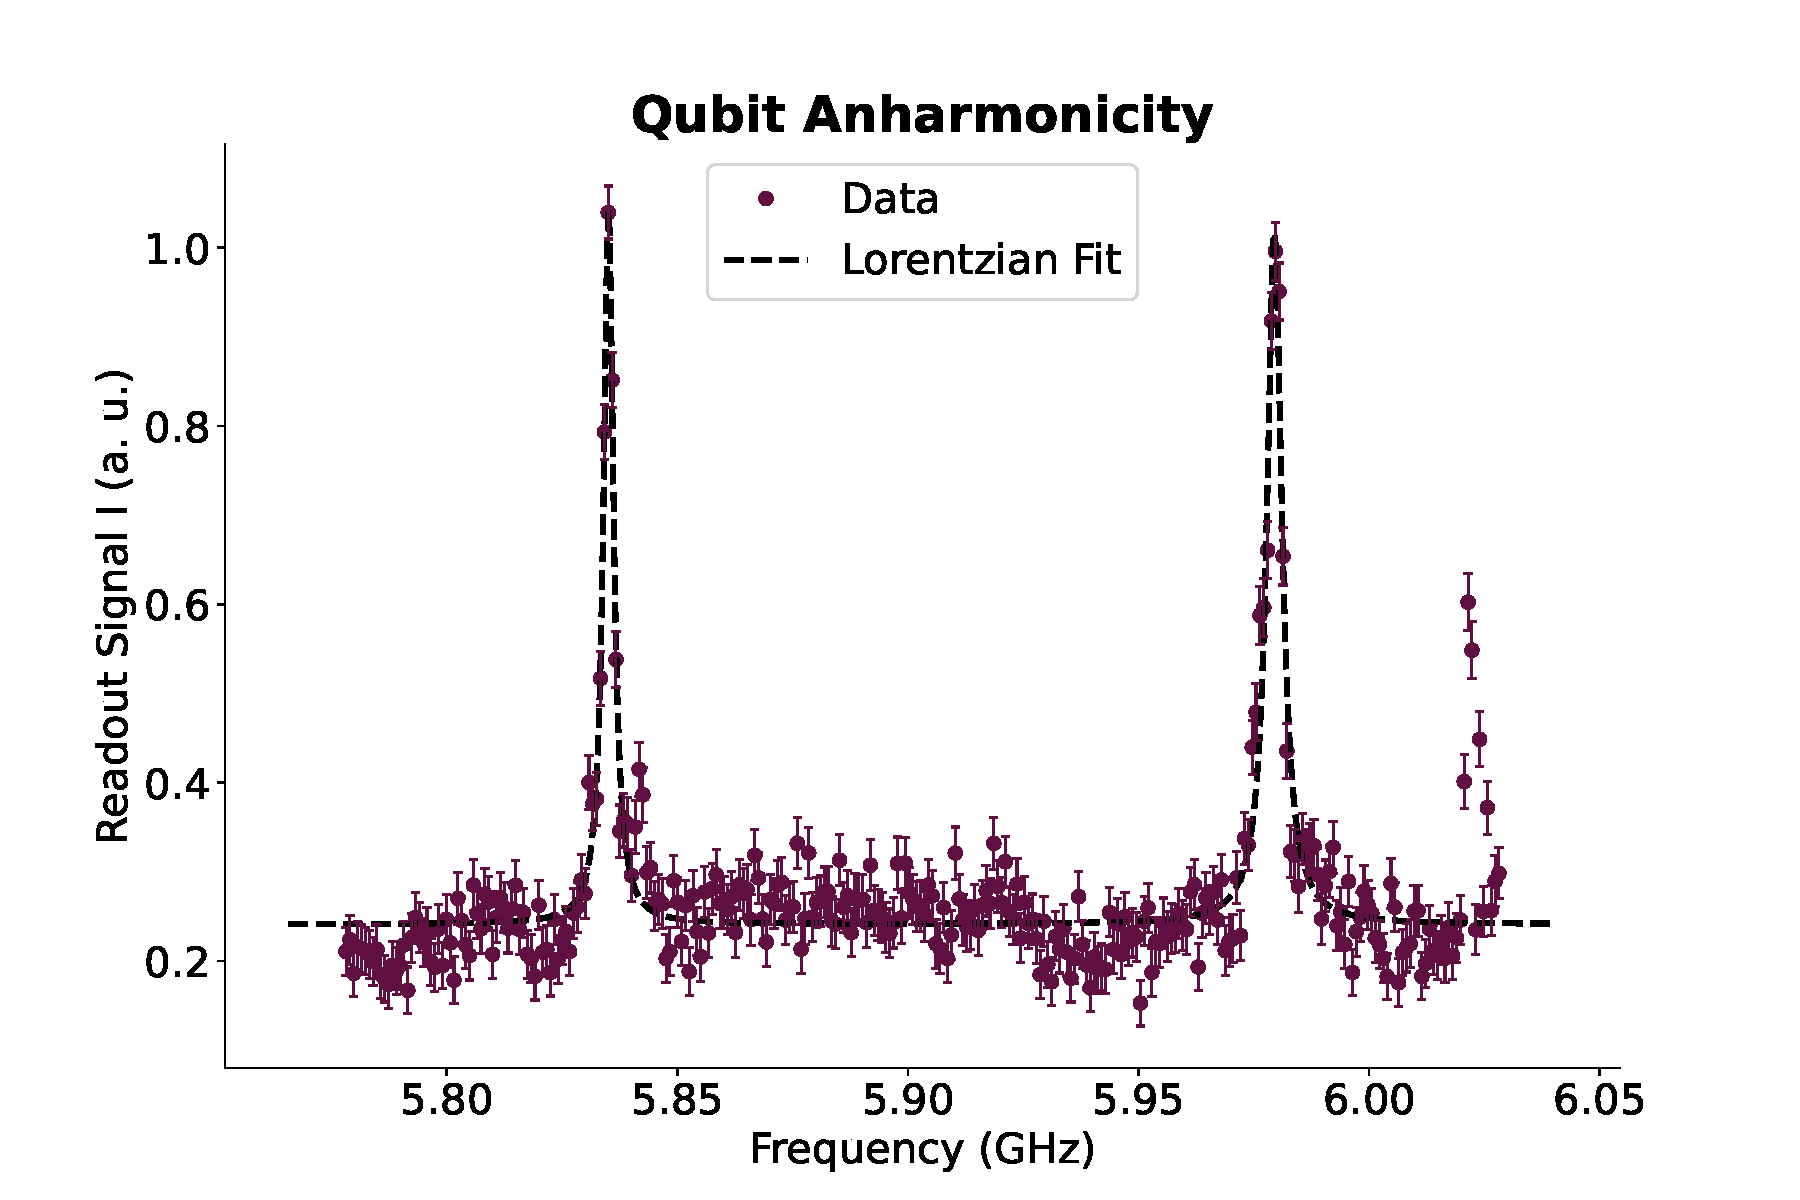
\includegraphics[width=1.0\linewidth]{Calibrations/Figures/Qubit Anharmonicity.pdf} % second figure itself
    \end{minipage}
    \label{fig:qubit_spectroscopy}
\end{figure*}
% \todo{Decide if we want to keep all the chi-squares. We can also make a big table in the appendix...}

From the two experiments, we can extract the qubit frequency and from the difference of the two, we get the anharmonicity. We extract the qubit frequency
\begin{equation}
    f_{01} = (5.98203 \pm 0.00008) \text{ GHz}
\end{equation}
And the anharmonicity is calculated as:
\begin{equation}
    \alpha = f_{02} - 2f_{01} = (-288.81 \pm 0.15) \text{ MHz}
\end{equation}
A comment worth making here is that the two-peak Lorentzian curve is not a good fit $\chi^2/\text{ndof} \approx 2.5$. This is largely due to an assumption that the background is constant. In general one should not trust the uncertainties of a poor fit, but to a large degree we do not need it here. If the main purpose was to determine the quantities to the best of our ability, we could have done more work here like fitting the two curves separately or continuing with other experiments were we could get even better estimates of the frequencies. In this thesis, we will suffice with a value "close to" the real value to make a realistic model.


\subsection{Rabi}
In section \ref{sec:how_to_make_gates}, we saw how one can make an x- and y-gates. With a known transition frequency and a set duration and envelope, we just lack the amplitude of the pulse to make sure the unitary evolution exactly corresponds to an $X$ or $Y$ gate. 
\begin{marginfigure}[5 cm]
    \centering
    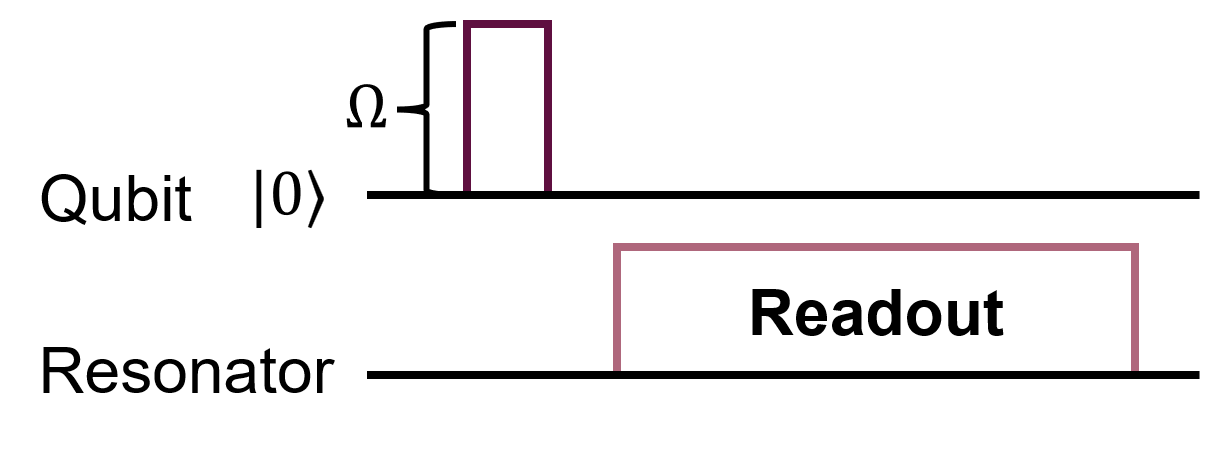
\includegraphics[]{Figs/circuits/rabi.png}
    \caption{The pulse sequence to determine the rabi amplitude. By varying the amplitude depicted with $\Omega$ and reading out the signal, the optimal $\Omega$ can be determined.}
    \label{fig:rabi_experiment}
\end{marginfigure}
The amplitude is determined by an experiment, where we initialize the qubit in state $\ket{0}$ and do a pulse with a frequency $\omega_d = \omega_q$ and amplitude $\Omega$ before reading it out. We will see oscillations depending on the area of the curve. Each top will correspond to a $\pi +n2\pi$ rotation around the $x$-axis, where the qubit will be in $\ket{1}$ and the bottoms will be at $2\pi n$ rotations, where the qubit is back in $\ket{0}$. With a cosine fit, we can pick the amplitude yielding us the $\pi$ rotation. To go from this pulse to a $\pi/2$ rotation, we can simply pick half of the $X_{\pi}$ amplitude \cite{Naglihou}. A schematic of the experiment is shown in figure \ref{fig:rabi_experiment} and the results from the experiment can be seen along with the cosine in figure \ref{fig:calibration_rabi}.
\begin{figure}
    \centering
    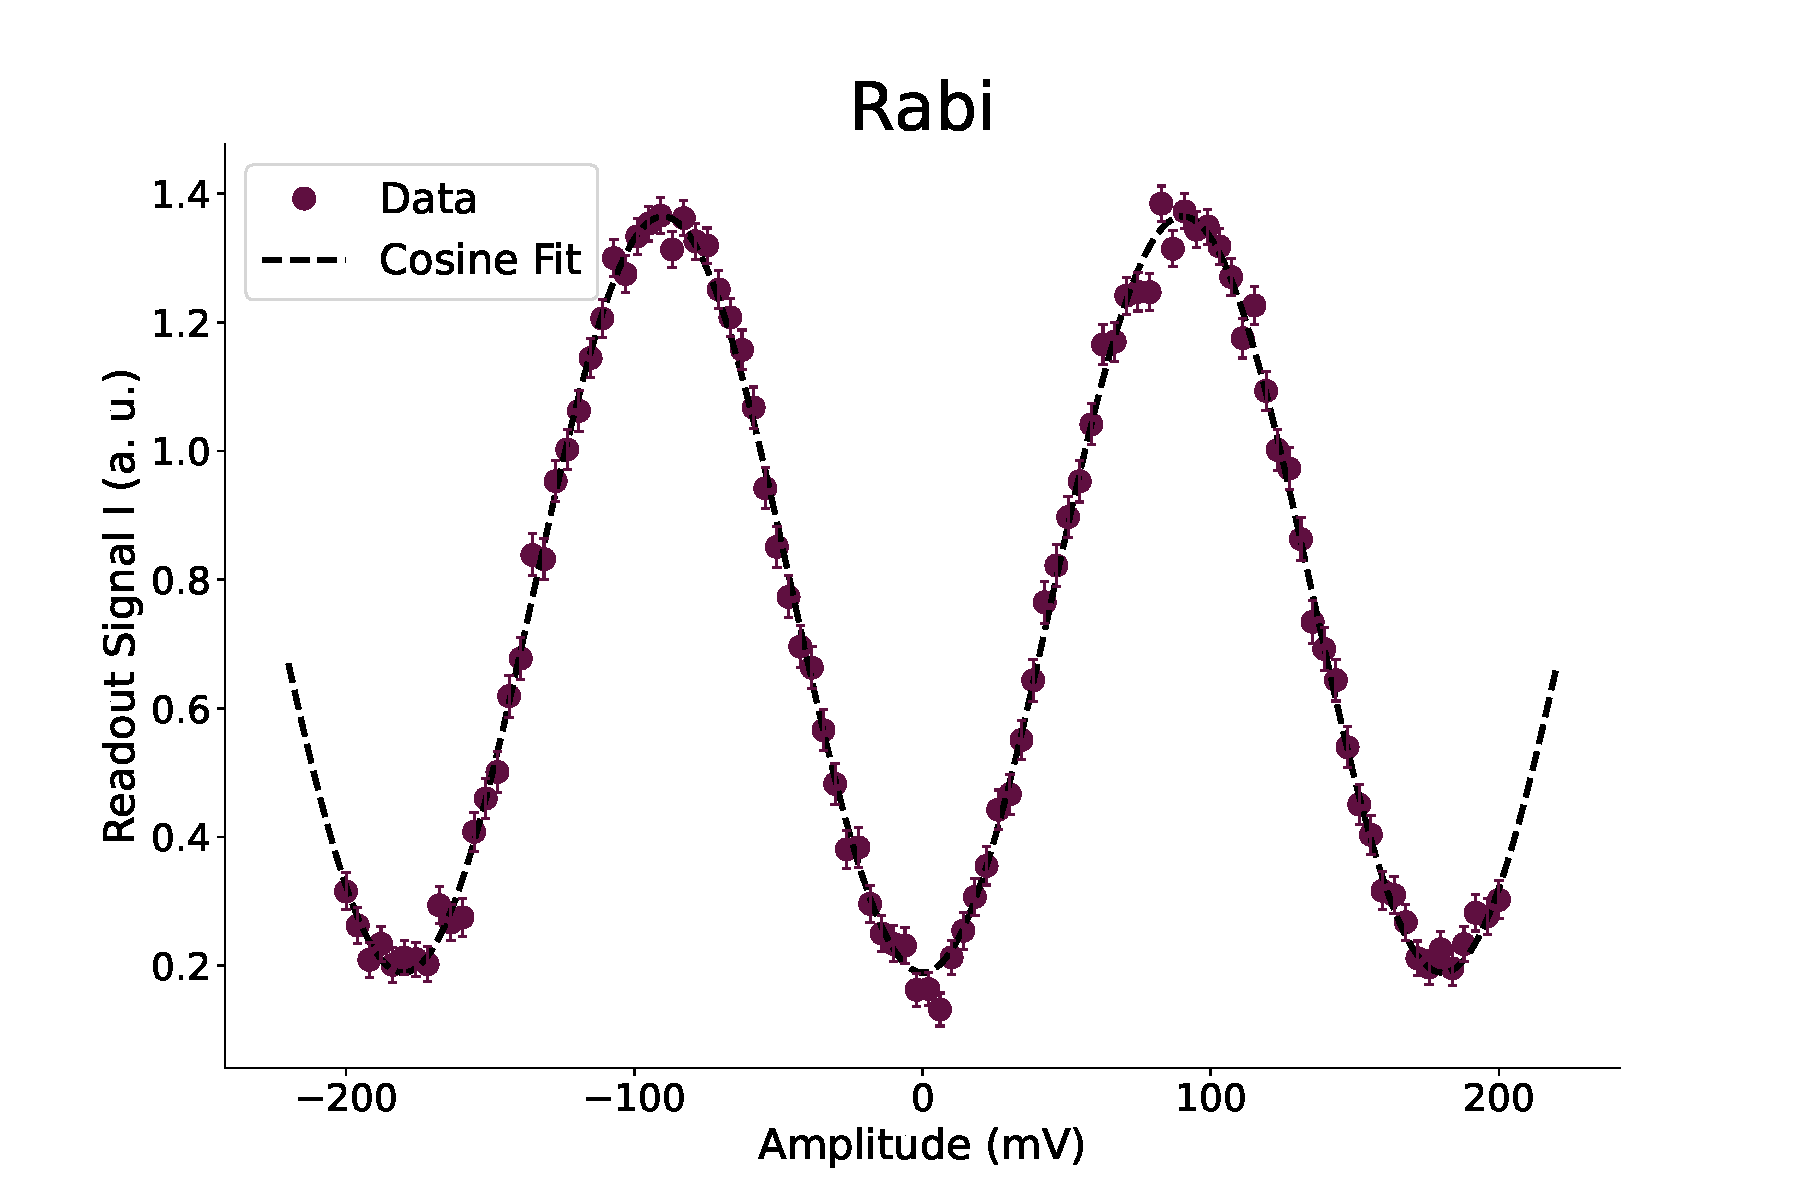
\includegraphics{Calibrations/Figures/Rabi.pdf}
    \caption{The outcome of a Rabi experiment. By varying the amplitude we get a cosine like behaviour which can be fitted to determine the top of the first wave. The curve is fitted with a function of the type: $y = A \cos(2 \pi x f + \phi) + b$ where x is the amplitude, y the outcome and $A, f, \phi$ and $B$ are the fitted parameters.}
    \label{fig:calibration_rabi}
\end{figure}

One could further improve the transition from $\ket{0}\to\ket{2}$ by applying envelopes derived from the DRAG scheme \cite{motzoi_simple_2009}. While these experiments are necessary to create an X-pulse and initilize our qubit in the $\ket{1}$ state, this calibration is not necessary for making the initialization in simulation, since we can just apply the x-gate directly. 

It is possible to determine the average fidelity of gates by a randomized benchmarking scheme \cite{knill_randomized_2008}. Without going into much depth, this was done to find an average gate fidelity of $F_{\text{gate}} = 0.9913 \pm 0.0003$. The infidelity contribution here will however be much lower than the other contributions from example temperature, so we will assume that we do a perfect X-gate in experiment. 


\subsection{Decay Calibration}\label{sec:calibration_t1}
\begin{marginfigure}[5 cm]
    \centering
    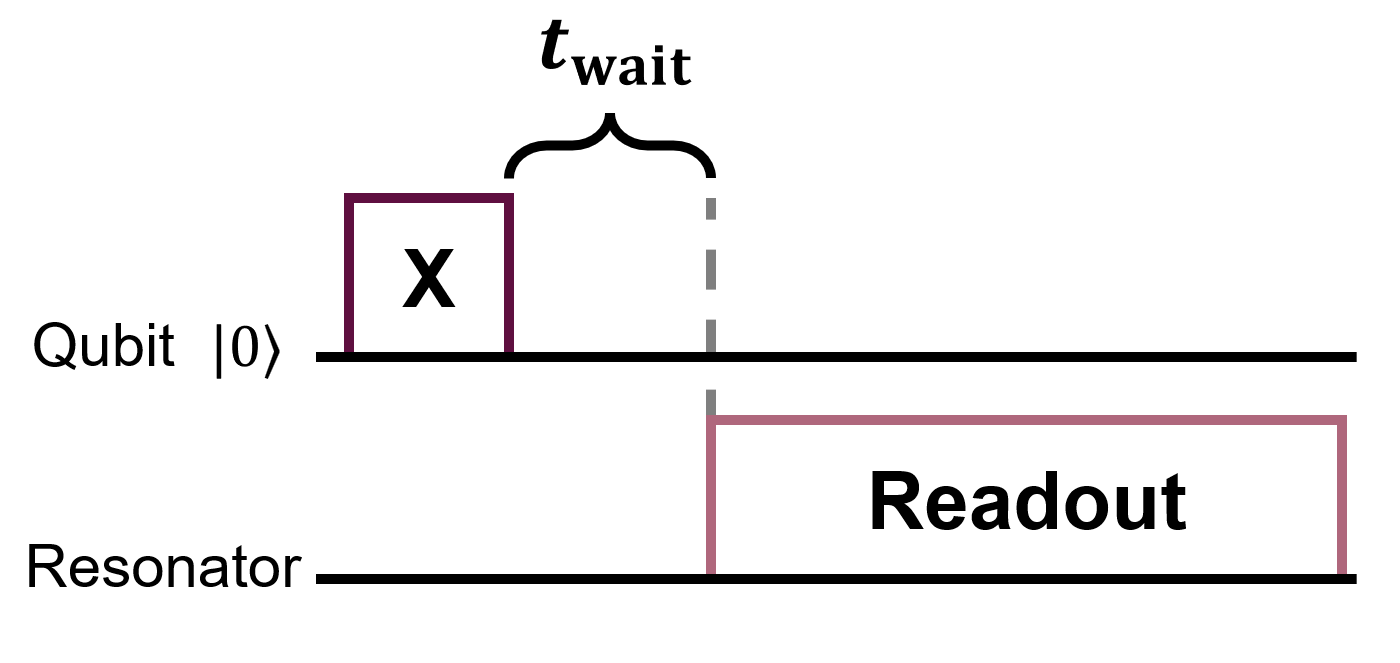
\includegraphics[]{Figs/circuits/t1.png}
    \caption{The pulse sequence used to do the $T_1$ calibration experiment.}
    \label{fig:t1_experiment_schematic}
\end{marginfigure}
In section \ref{sec:theory_t1}, we saw that the characteristic longitudinal decay time, $T_1$ determines the relationship between $\rho_{00}(t)$ and $\rho_{11}(t)$. For this experiment, we will initialize the qubit in state $\ket{1}$ since this state is the furthers from the steady state. We then wait some time $t_{\text{wait}}$ before measuring the qubit. By repeating this experiment multiple times for different waiting times (see figure \ref{fig:t1_experiment_schematic}), we can approximate  $\rho_{00}(t)$ and $\rho_{11}(t)$ by taking the average at each time step. Now plotting the occupation as a function of time, we will obtain a decaying function going toward the steady state. The exponential coefficient of this decay is given by $1/T_1$ \cite{krantz_quantum_2019}. 

Doing the experiment on our qubit, we obtain the results displayed in figure \ref{fig:calibration_T_1_decay}. The exponential fit gives the value for $T_1$:
\begin{equation}
    T_1 = (4.30 \pm 0.12) \text{ µs}
\end{equation}

\begin{figure}
    \centering
    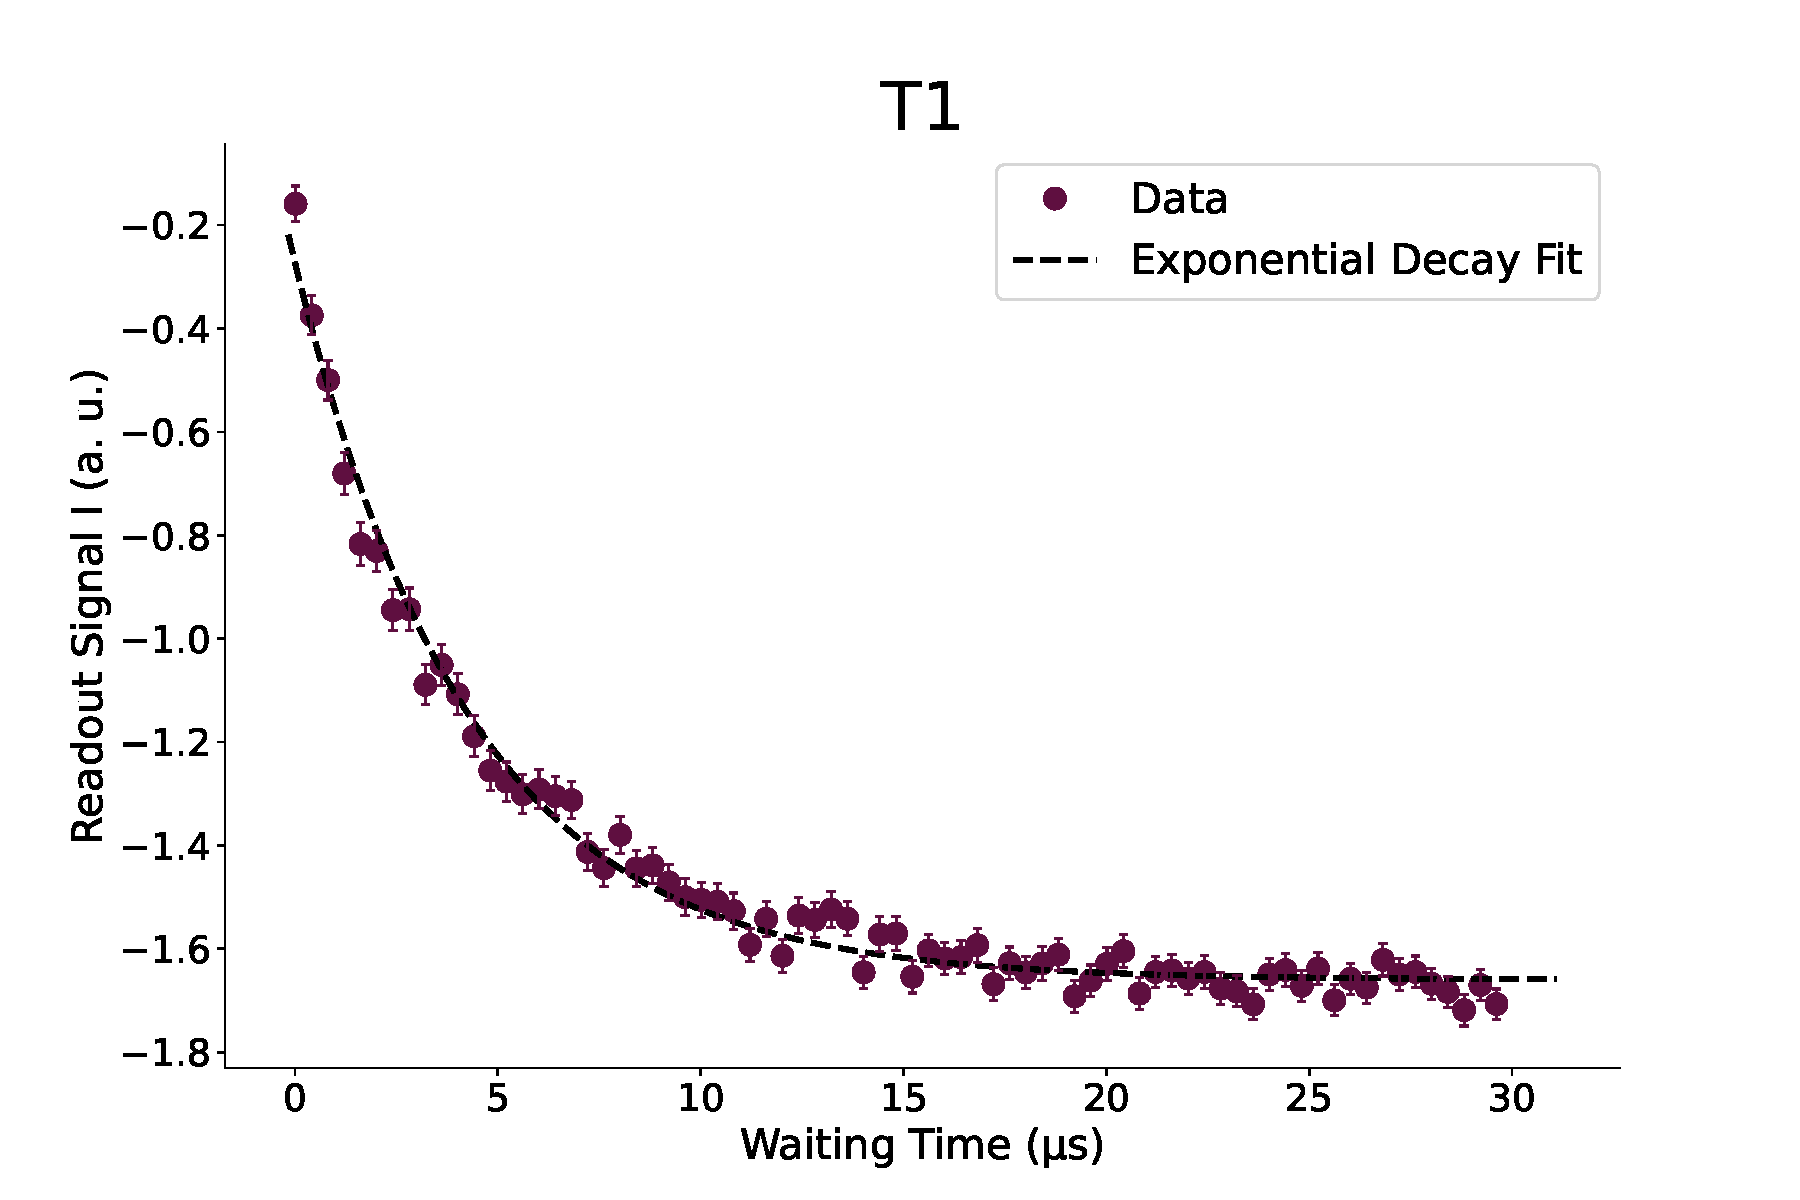
\includegraphics[]{Calibrations/Figures/T1.pdf}
    \caption{Data from an experiment determining the characteristic $T_1$ decay time. The fit is an exponential decay given by: $y = A e^{-t / T_1} + b$ where $t$ is the waiting time, $y$ is the outcome of the experiment and $A, b$ and $T_1$ are fit parameters.}
    \label{fig:calibration_T_1_decay}
\end{figure}

The $T_1$ comes from interaction between qubit and environment which unfortunately changes over time. This leads to a fluctuating $T_1$ time, so even though one can determine the current $T_1$ with a high precision, it might change just few hours later. This experiment was run just seconds before the readout sequence described in \ref{chap:readout}. But in section \ref{sec:continuous_calibratino}, we will see that an experiment done on the same device just a few months before will have significantly higher $T_1$. To see an example of $T_1$ fluctuations of our device over just a few hours, see figure \ref{fig:changing_t1}.
\begin{marginfigure}[-5 cm]
    \centering
    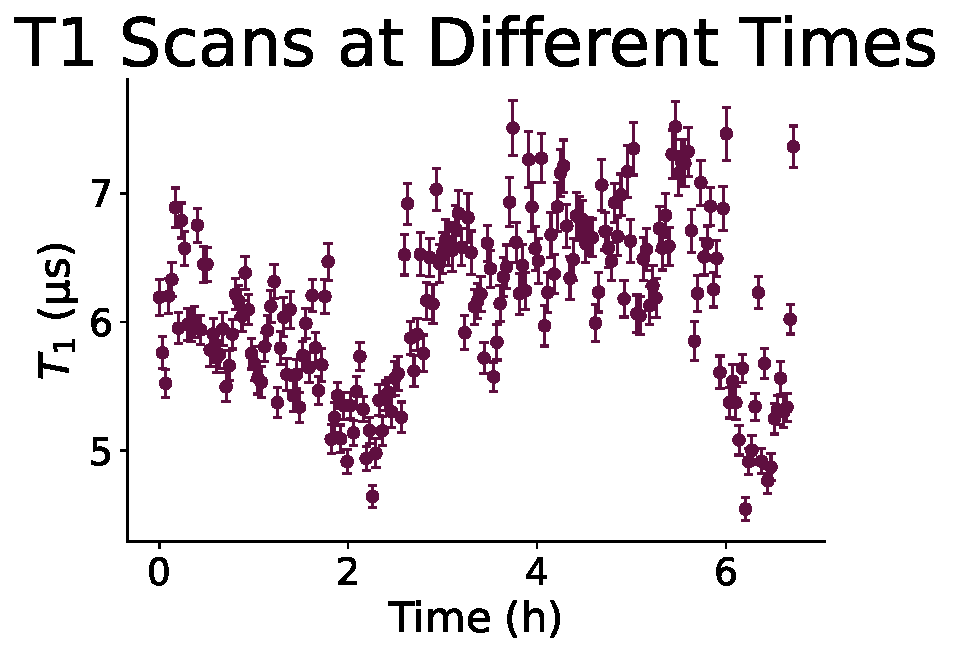
\includegraphics[]{Calibrations/Figures/T1 Scans at Different Times.pdf}
    \caption{The results from repeated $T_1$-calibrations over a few hours. }
    \label{fig:changing_t1}
\end{marginfigure}

\subsection{Dephasing Calibration}
\begin{marginfigure}
    \centering
    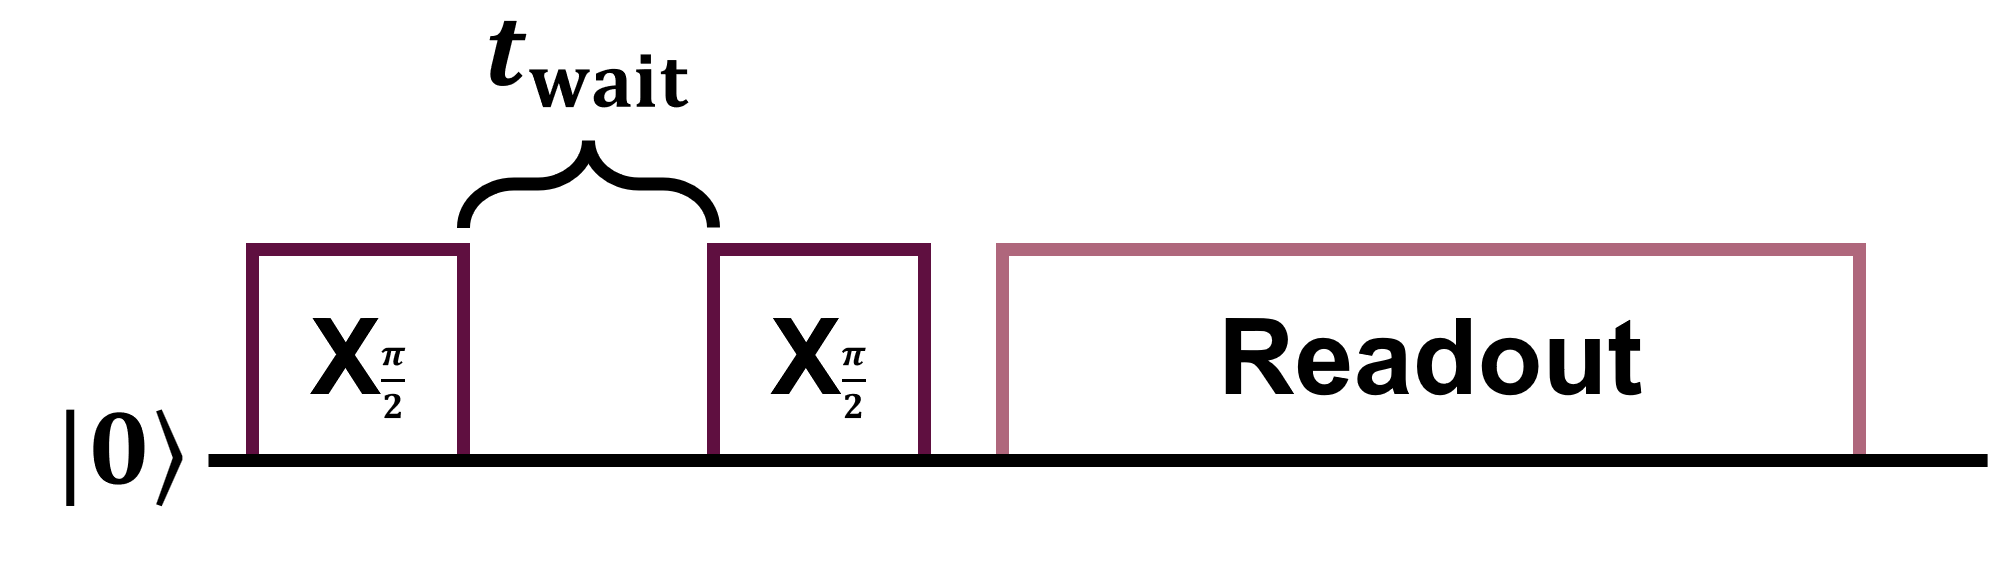
\includegraphics{Figs/circuits/t2.png}
    \caption{Ramsey experiment schematic. Two $X_{\pi/2}$ pulses intentionally detuned from the qubit frequency are applied with a wait time in between them. Afterwards the qubit is measured by performing a readout pulse on the resonator.}
    \label{fig:enter-label}
\end{marginfigure}
The dephasing of the qubit is not as important a parameter when we look at readout. For completeness and because we also make use of dephasing in the efficiency calibration in section \ref{sec:readout_efficiency}, we will still do a calibration. To measure $T_2$, one does a Ramsey style experiment, where a pulse with a frequency slightly offset from the qubit frequency (in our case $5 \text{ MHz}$ is applied to perform an $X_{\pi/2}$ pulse. This state will now start to precess around the $z$-axis. After some time the pulse is performed again. This leads time-dependent oscillations which are dependent on the state of the qubit when performing the second pulse. In addition, the qubit will experience dephasing while at the equator of the Bloch sphere, leading it to a mixed state. This gives an almost exponential envelope of the oscillations where the exponential coefficient is determined by the $T_2$ time \cite{krantz_quantum_2019}.

\begin{figure*}[t]
    \begin{minipage}{0.50\linewidth}
        \centering
        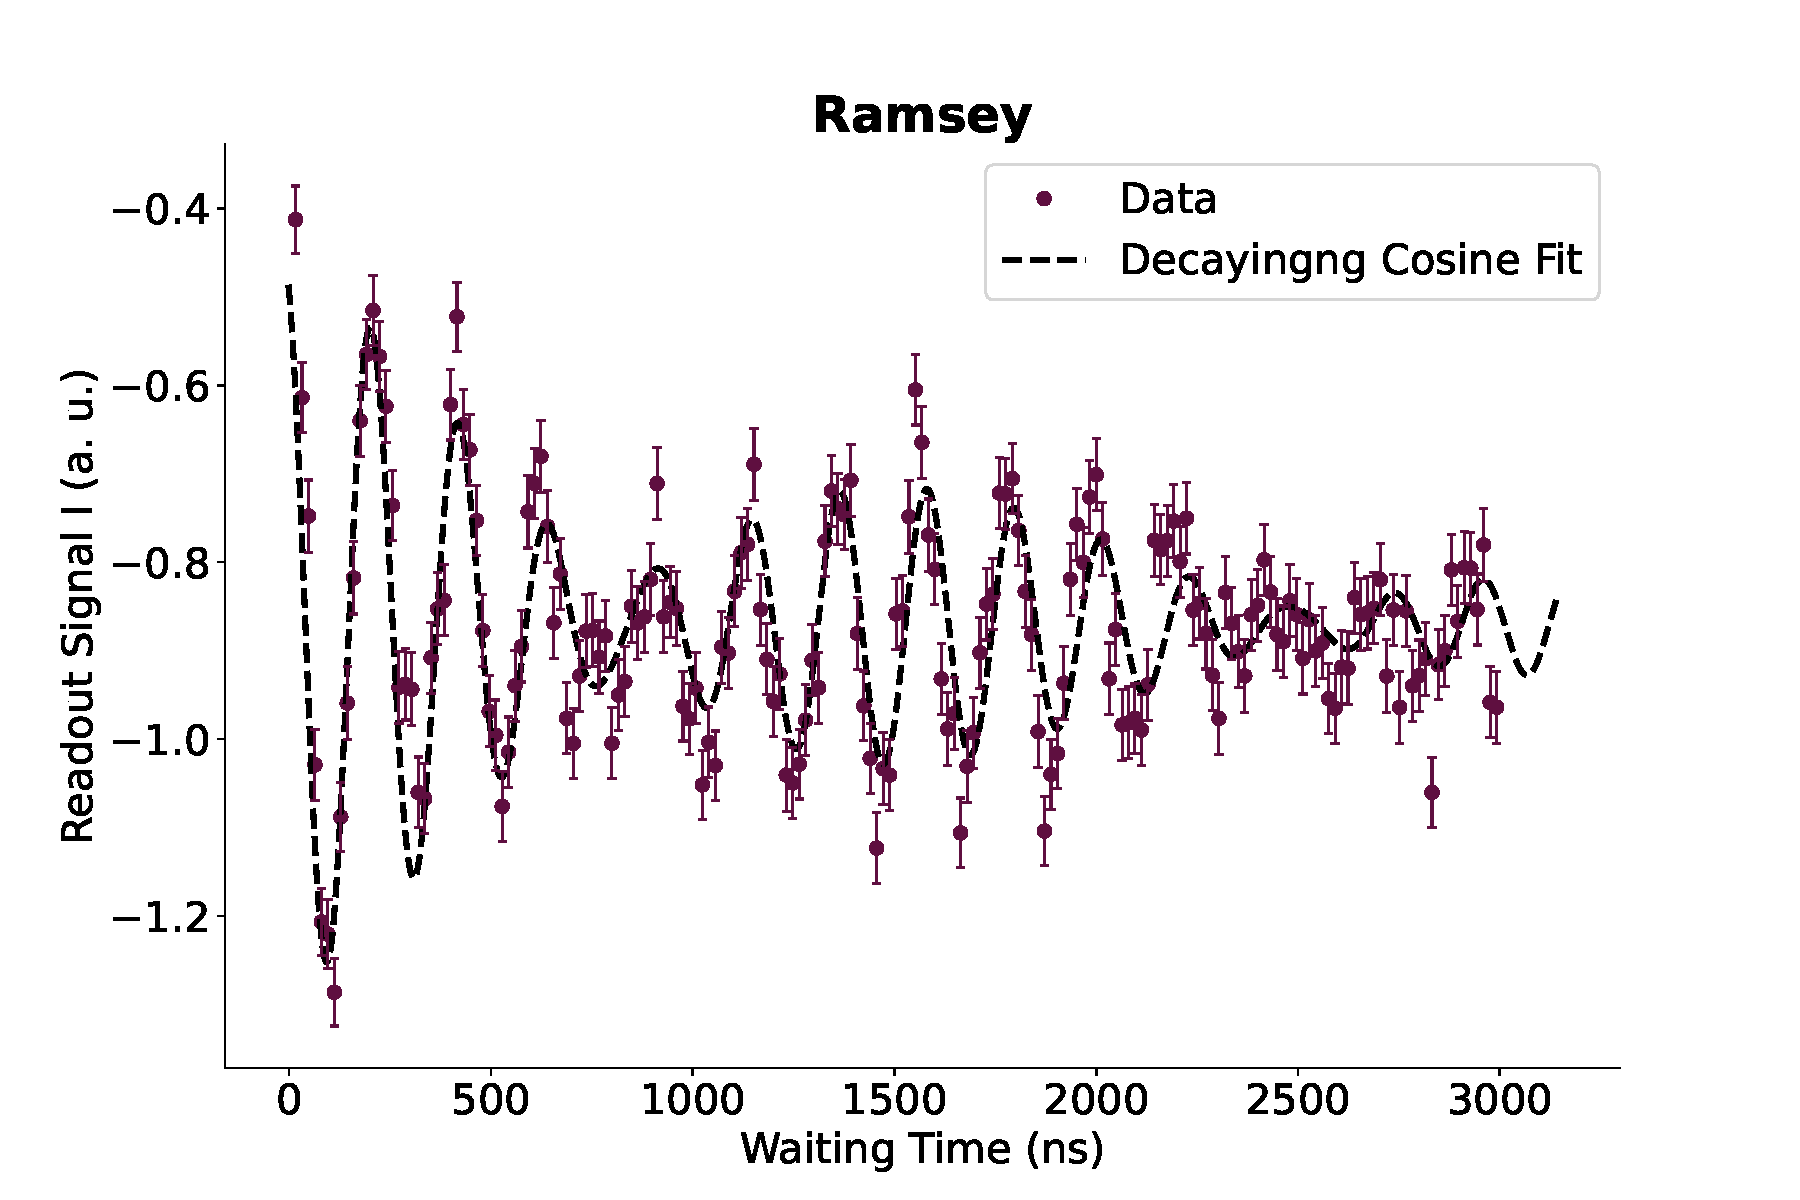
\includegraphics[width=1.0\linewidth]{Calibrations/Figures/Ramsey.pdf} % first figure itself
    \end{minipage}
    \begin{minipage}{0.50\linewidth}
        \centering
        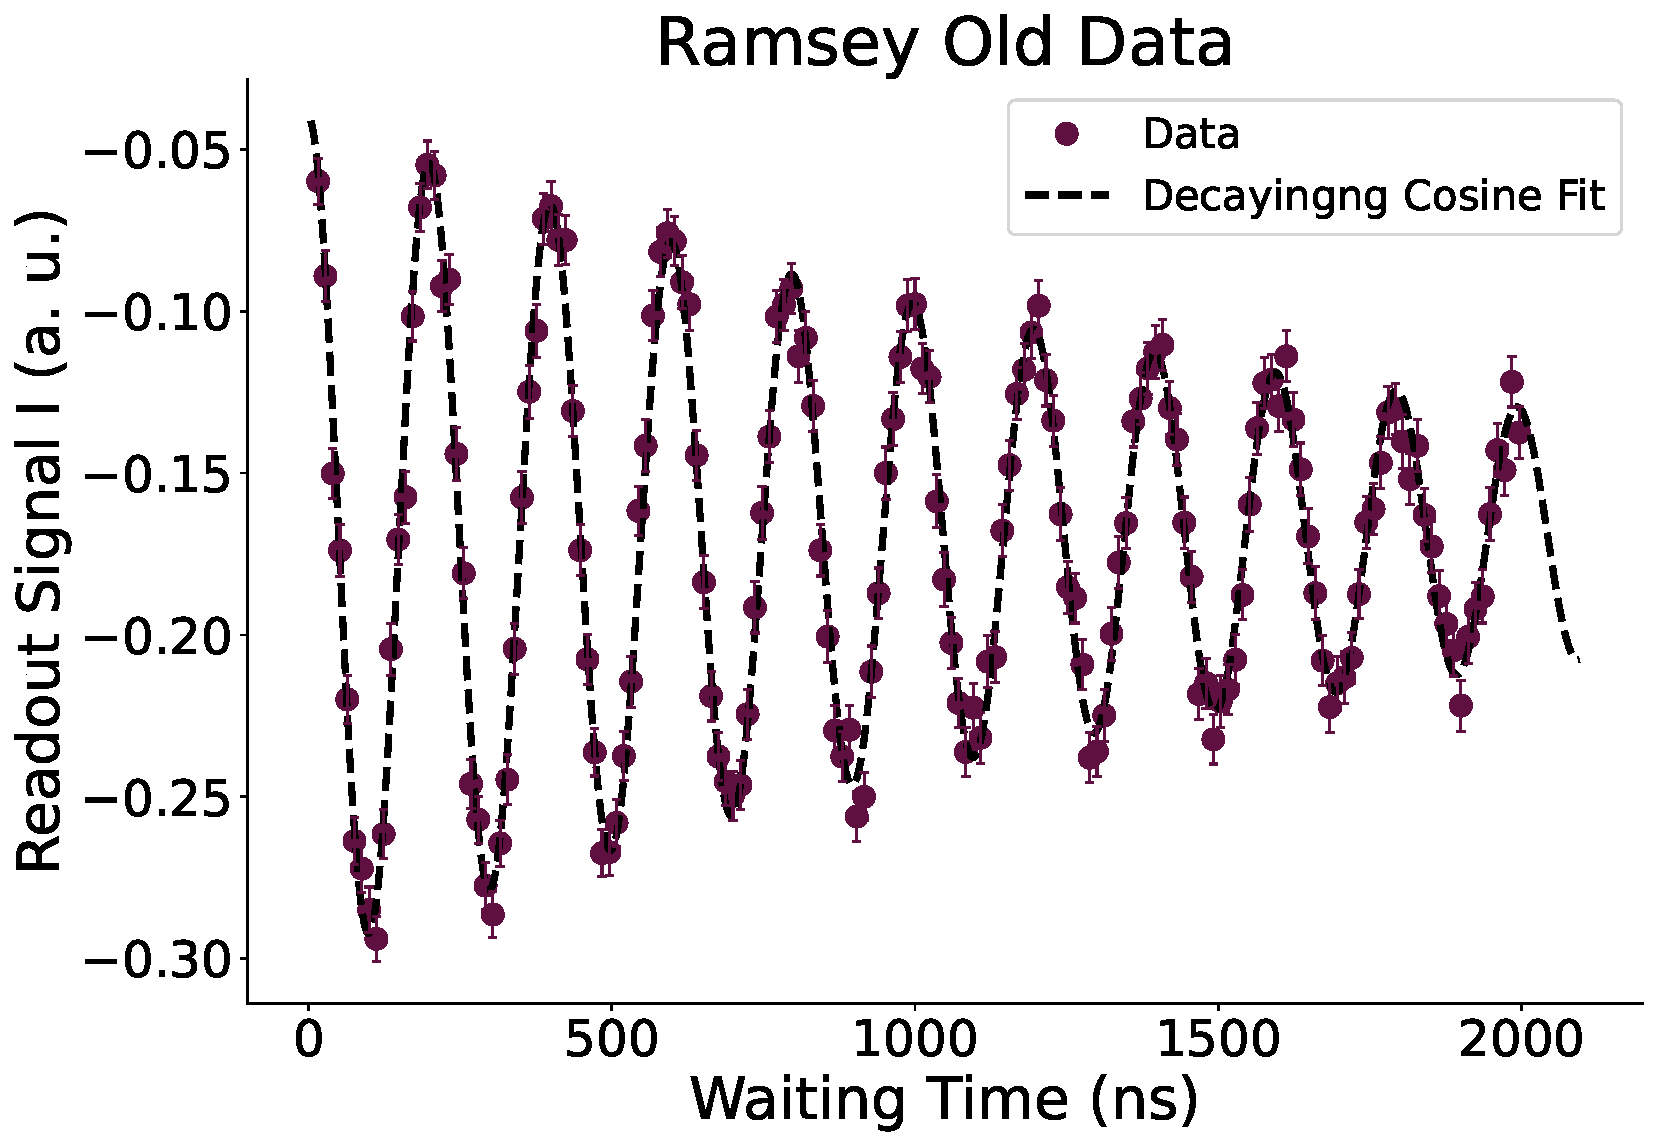
\includegraphics[width = 1.0 \linewidth]{Calibrations/Figures/Ramsey Old Data.pdf}        
    \end{minipage}
    \caption{Figures showing the T2 experiment. The left shows the Ramsey $T_2$ while the right shows an older $T_2$ experiment on the same device. Both are fitted with a function of the type $y = A \cos(2 \pi t f + \phi) e^{-t / T_2} + b$ where $t$ is the waiting time, $y$ is the outcome and $f, \phi, A, b$ and $T_2$ are fitting parameters. An additional cosine pulse is added to the left one adding the parameters $f_1, \phi_1, A_1$.}
    \label{fig:calibrations_t2}
\end{figure*}
In figure \ref{fig:calibrations_t2} two Ramsey experiments are shown. The left one was done before the measurement and the right is a few weeks older. It was run with the same parameters on the same device but this just displays the sensitivity to changes in environment. In the left one, we allowed for two cosine oscillation terms, since we suspect that the system couples to another two level system leading to additional oscillation. The envelope give us:
\begin{equation}
    T_2 = (1.65 \pm 0.12) \text{ µs} 
\end{equation}
Which can further give us the dephasing time, by using equation \ref{eq:t2_equation}:
\begin{equation}
    T_\phi = \left(\frac{1}{T_2} - \frac{1}{2T_1} \right)^{-1} = (1.38 \pm 0.08) \text{ µs}
\end{equation}
Where we again should be careful about using this as more than an estimate because of the data does not fit our initial model. 

% \paragraph{Echo Experiememt*}
% This is the limit if we allow activly chanigning the qubit to echo out the phases. We can thus eliminate low frequency noise.

% \begin{equation}
%     T_2^* = (2.85 \pm 0.09) \text{ µs} 
% \end{equation}
% \todo{Need somw good discussion here. This $T_2$ is just important when we do the efficiency calibration it is not important in simulation.}


\section{Resonator Calibration}
With the qubit calibrated, we will move on to the resonator. The resonator is modelled as a quantum harmonic oscillator, so the non-interacting Hamilton is completely determined by its frequency, $f_r$. However, the interaction with the qubit required us to calibrate the dispersive shift and the coupling strength $g$. To model the coupling to its environment we determine the photon dissipation rate $\kappa$,  and lastly we will estimate steady state photon number, $\Bar{n}_{\text{ss}}$ which is closely related to the amplitude of the drive pulse, $\epsilon$.

\subsection{Spectroscopy}
Like the qubit, we can perform resonator spectroscopy to find the frequency. Because of the dispersive interaction (described in section \ref{sec:dispersive_regime}, we will get a different frequency when the qubit is in $\ket{0}$ or in $\ket{1}$ and we will have to do the experiment with both initialization. Since the the photons in the resonator have an exponential lifetime, the frequency spectrum will have Lorentzian curve around the resonance frequency. The experiment and the associated fits can be seen in figure \ref{fig:spectroscopy_resonator}. Since $\ket{1}$ decays to $\ket{0}$ in many cases, we have added a second Lorentzian to the fit of resonator when the qubit is excited state. In addition, we have limited the fitting points to be around the peak, since the background is not constant but also have some oscillations which we contribute to a finite-size demodulation window \cite{resonator_spectroscopy}.
\begin{figure}
    \centering
    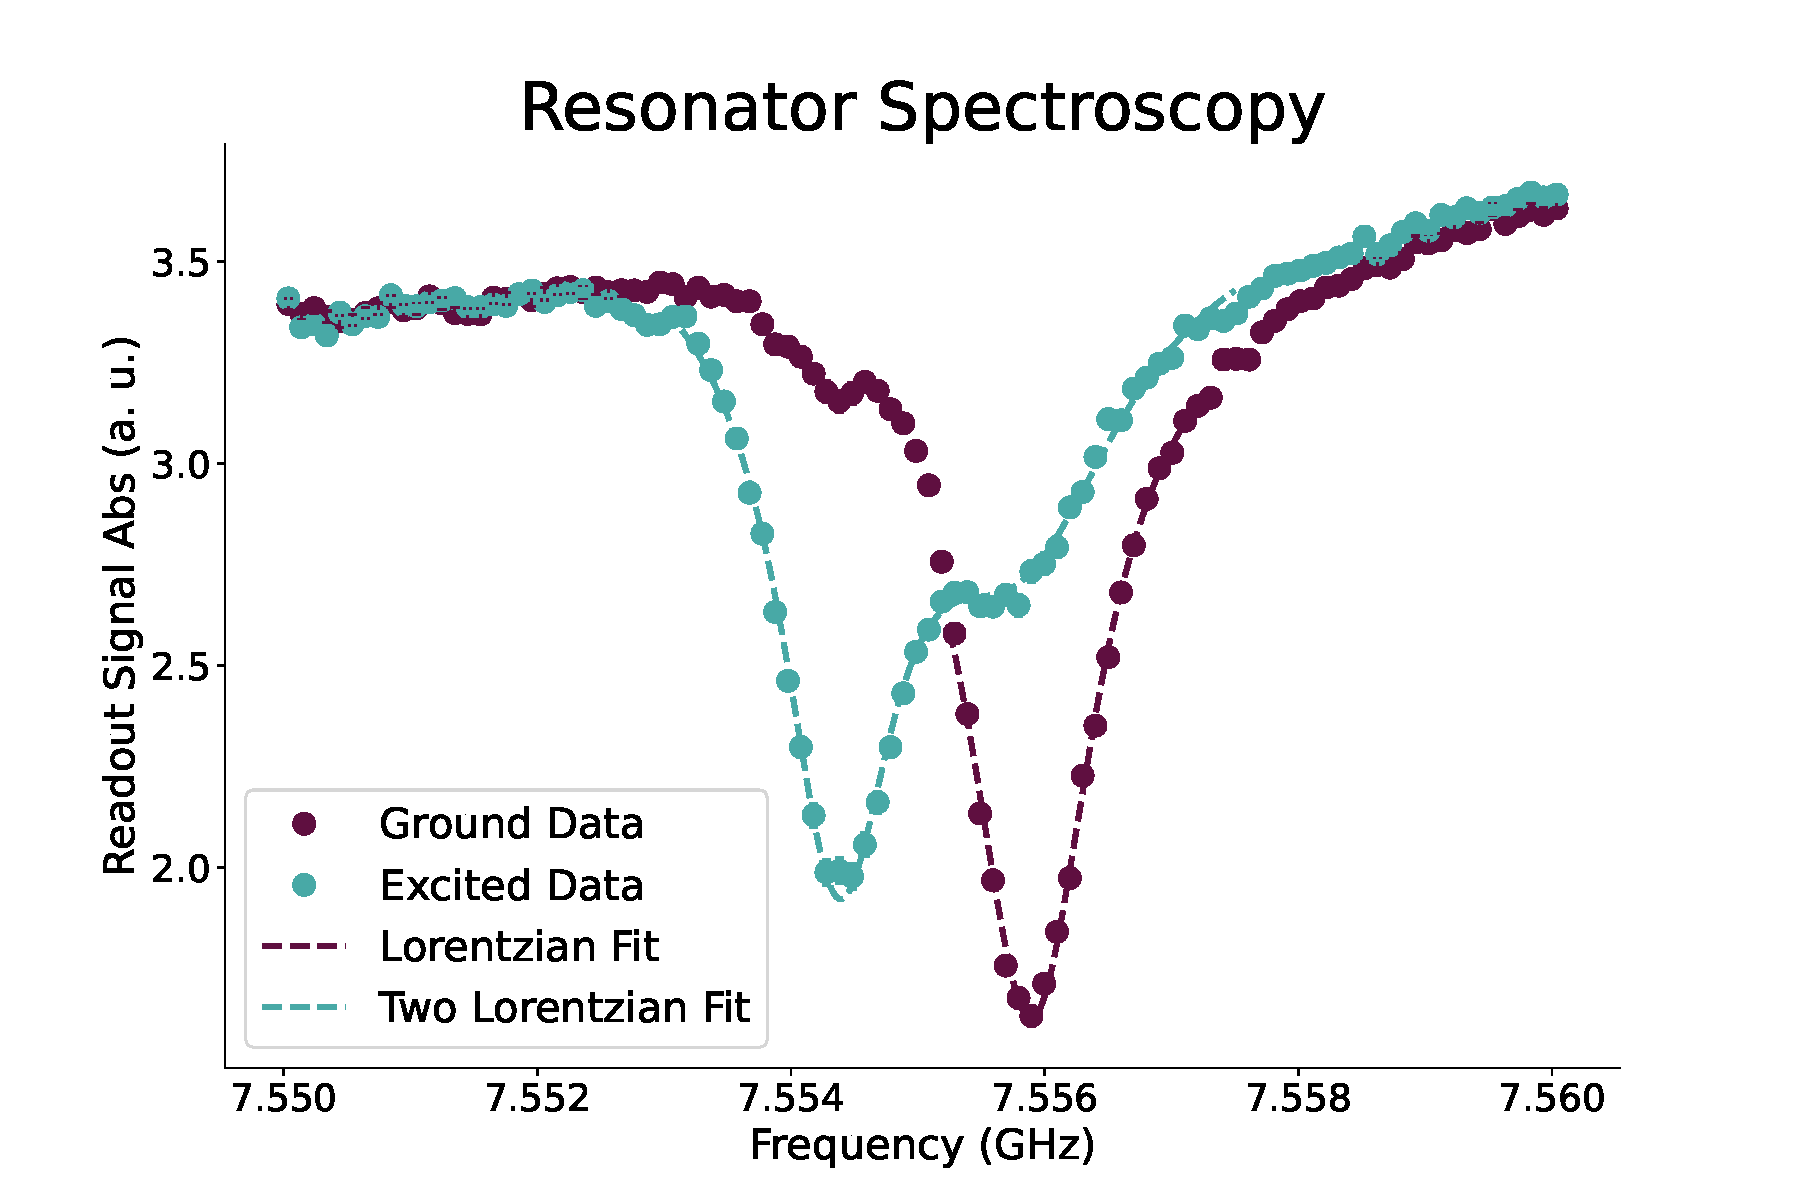
\includegraphics{Calibrations/Figures/Resonator Spectroscopy.pdf}
    \caption{Spectroscopy of the resonator signal where the qubit is either in $\ket{0}$ (purple) or in $\ket{1}$ (light blue). Since $1$ is somewhat decayed into $0$, the curve for $1$ is fitted with two Lorentzians.}
    \label{fig:spectroscopy_resonator}
\end{figure}
The two frequencies come out to be:
\begin{equation}
     f_{r0} = 7.55590 \text{ GHz} \pm 3 \text{ KHz} ;\quad f_{r1} =  7.55439 \text{ GHz} \pm 7 \text{ KHz}
\end{equation}
For these parameters, we can extract the resonator frequency $f_r$ and the dispersive shift $\chi$. This can further be used together with the resonator-qubit detuning to calculate the coupling between qubit and resonator in the dispersive approximation using equation \ref{eq:chi}:
\begin{align}
    f_r  = (f_{r0} + f_{r1}) / 2 &= 7.555130 \text{ GHz} \pm 4 \text{ KHz} \\
    \chi = (f_{r0} - f_{r1}) / 2 &= (763.5 \pm 4) \text{ Khz}  \label{eq:dispersive_shift}\\
    g    = \sqrt{\chi (f_r - f_q)\left(1 + \frac{f_r - f_q}{\alpha}\right)} &= (87.0 \pm 0.4) \text{ MHz}
\end{align}
Such that we now can calculate both the resonator Hamiltonian and the full interacting one.

\subsection{Resonator Decay Rate}
To model the resonator dissipation, we will now calibrate $\kappa$. We found in section \ref{sec:resonator_decays} that the resonator will decay exponentially when not driven. With this information, we can find $\kappa$ by simply filling the resonator and watching it deplete. By applying a pulse untill steady state is reached and monitoring the $I, Q$ signal during depletion, we can get the trajectory of mean photon count\footnote{Up to a factor which we is not needed to determine the exponential factor}. An average of 10,000 trajectories are performed of this and the average trace is demodulated and also course grained in $10 \text{ ns}$ intervals to reduce the noise. The results along with an exponential fit of the depletion can be seen in figure \ref{fig:calibration_of_kappa}. The exponent factor is found to be:
\begin{figure}[h]
    \centering
    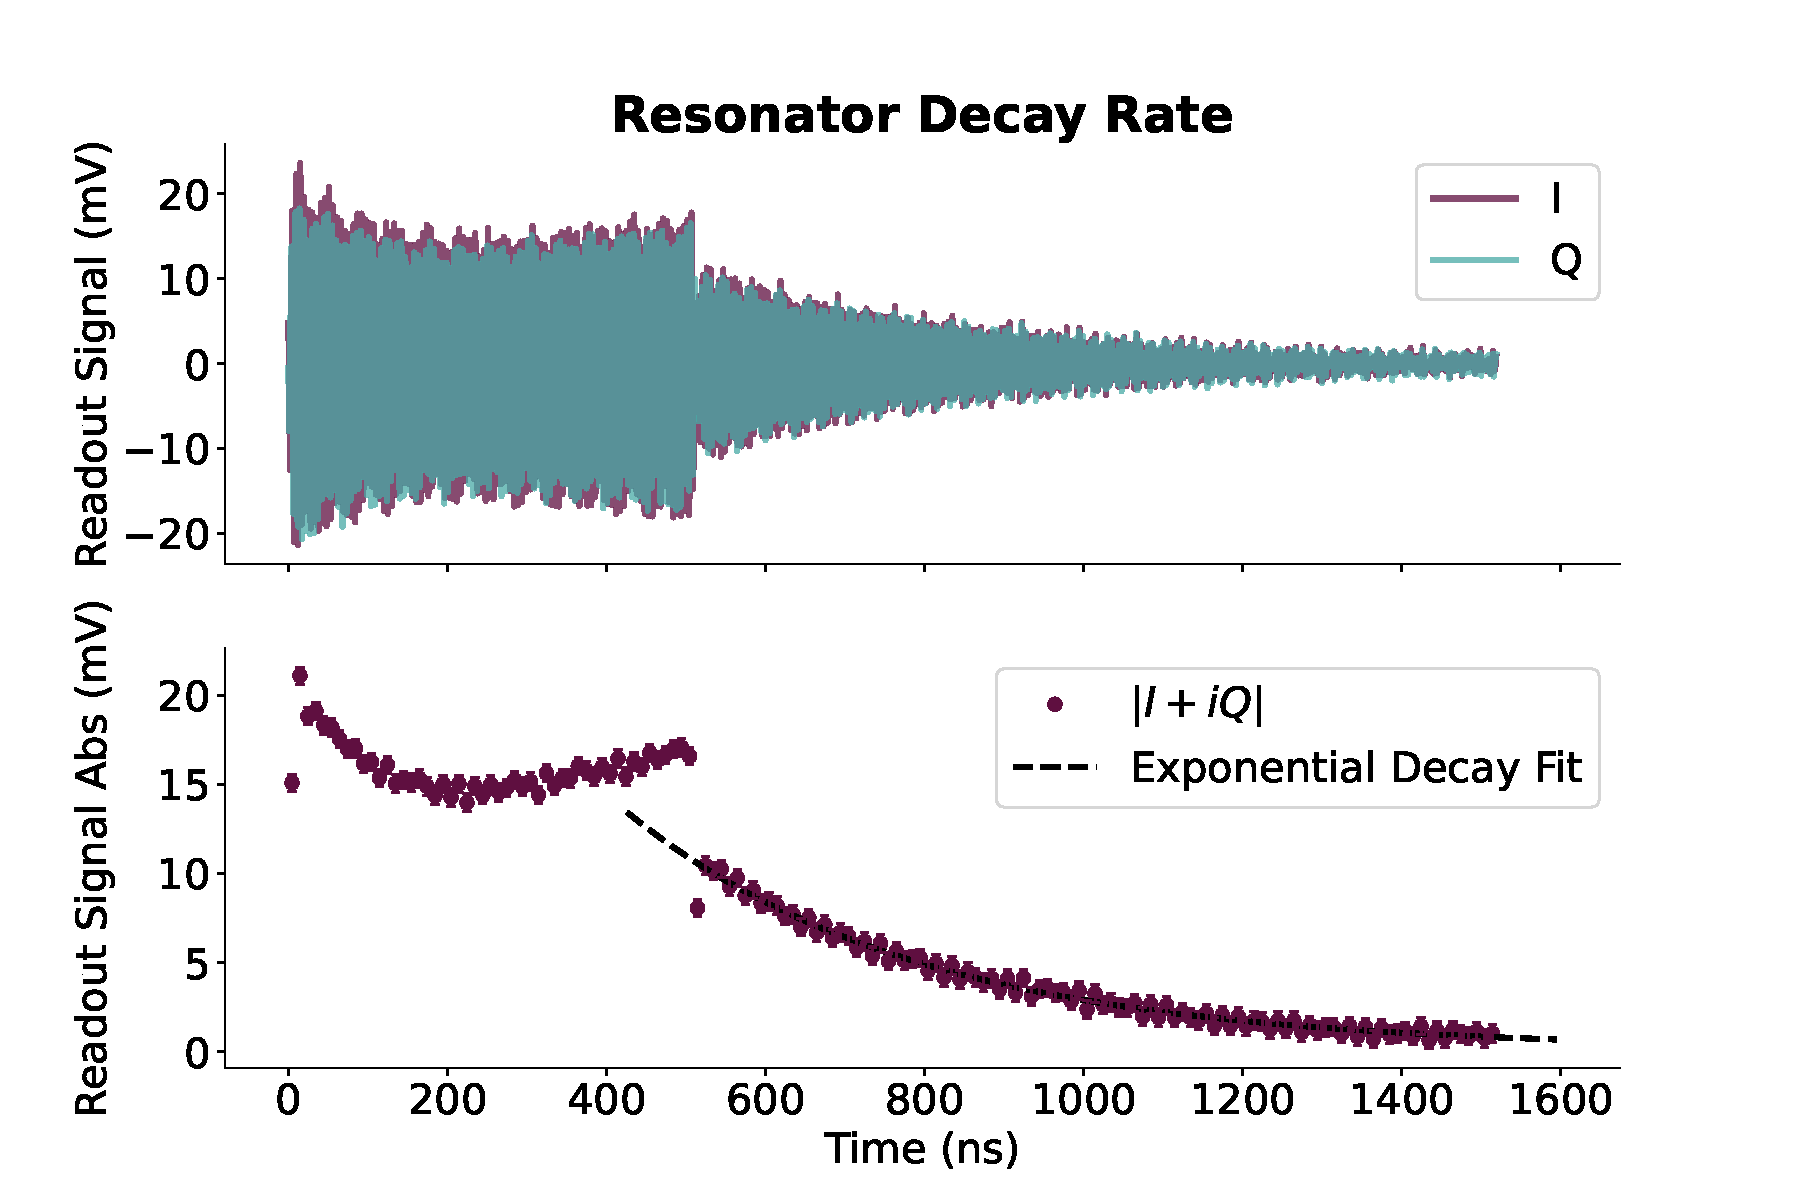
\includegraphics{Calibrations/Figures/Resonator Decay Rate.pdf}
    \caption{Traces from a short drive and a following monitoring of the feed line. In the top panel, the meaned $IQ$ traces are taken. In the lower, the $|I(t) + iQ(t)|$ values are plotted and averaged over $10 \text{ ns}$ intervals. The last part (from $t = 600 \text{ ns}$ is fitted with an exponential function: $y = Ae^{-\kappa t} + b$ where $t$ is the time $y$ is proportional to the mean photon number and $A, b$ and $\kappa$ are fitting parameters.}
    \label{fig:calibration_of_kappa}
\end{figure}
% After it is sufficiently excited, we stop the pulse but continue to monitor the $I$ and $Q$ signal. Remembering that the average photon number can be found from the distance to origo in the $I-Q$-plane, we plot $\Bar{n}(t) = |I(t)+iQ(t)|$. An average of 10,000 trace from this experiment is displayed in \ref{fig:calibration_of_kappa}. The traces are coarse grained over a $10 \text{ ns}$ interval to cancel some unwanted oscillating behaviour. Fitting the last part of the data, we obtain:
\begin{equation}
    \kappa = 3.8 \pm 0.6 \text{ MHz}
\end{equation}
We can also compare this to the width of the resonator dips. With the Lorentzian distribution the width is given as $2 \pi \kappa$ \cite{krantz_quantum_2019}. From the fits above calibrating the resonator frequency, we find  $\kappa = (3.87 \pm 0.08) \text{ MHz}$ when the qubit is in $\ket{0}$ and $\kappa = (3.50 \pm 0.07) \text{ MHz}$ from $\ket{1}$. For $\ket{1}$ some of the dynamics will however mix with $T_1$ decay of the qubit and is not as reliable.   

\subsection{Photon Counting}
To recreate the simulation, we will now need to calibrate the pulse as well. In the experiment, it is determined by some voltage, which we will have to convert to coupling operator going into the Hamiltonian with units of energy. To do this, we will calibrate the amount of photons present in the steady state. This will be done using the two properties:
\begin{enumerate}
    \item In section \ref{sec:resonator_decays}, we described how the resonator goes into a steady state when driven. In the IQ plot, the mean photon number was proportional to the driving amplitude. 
    \item Like the qubit state shifts the resonator frequency, the qubit frequency is also shifted in we were to fill the resonator with photons. We can use this to rewrite equation \ref{eq:dispersive_shift_tls} to the convenient form: $H = \Tilde{\omega}_r a^\dagger a  + \left(\frac12 \Tilde{\omega}_{01} + \chi a^\dagger a\right)  \sigma_z$
\end{enumerate}
We can now calibrate the photon count in its steady state by driving the resonator until the steady state is reached. Then we do a qubit spectroscopy experiment like the one in \ref{sec:qubit_spectroscopy} to determine the effective qubit frequency. We then repeat the experiment at multiple amplitudes of resonator pulse and multiple frequencies for the qubit pulse. By fitting a second order polynomial we can interpolate the shift at the driving strength $\epsilon$ and divide it with the dispersive shift to estimate the mean photon number in the resonator steady state. The experiment is visualized in figure \ref{fig:photon_counting_circuit}. The results for the scan can be seen in the top panel of figure \ref{fig:calibration_photon_counting_scan}, whereas the lower panel shows the calculation of mean photon number at different amplitudes.  
\begin{marginfigure}[-4 cm]
    \centering
    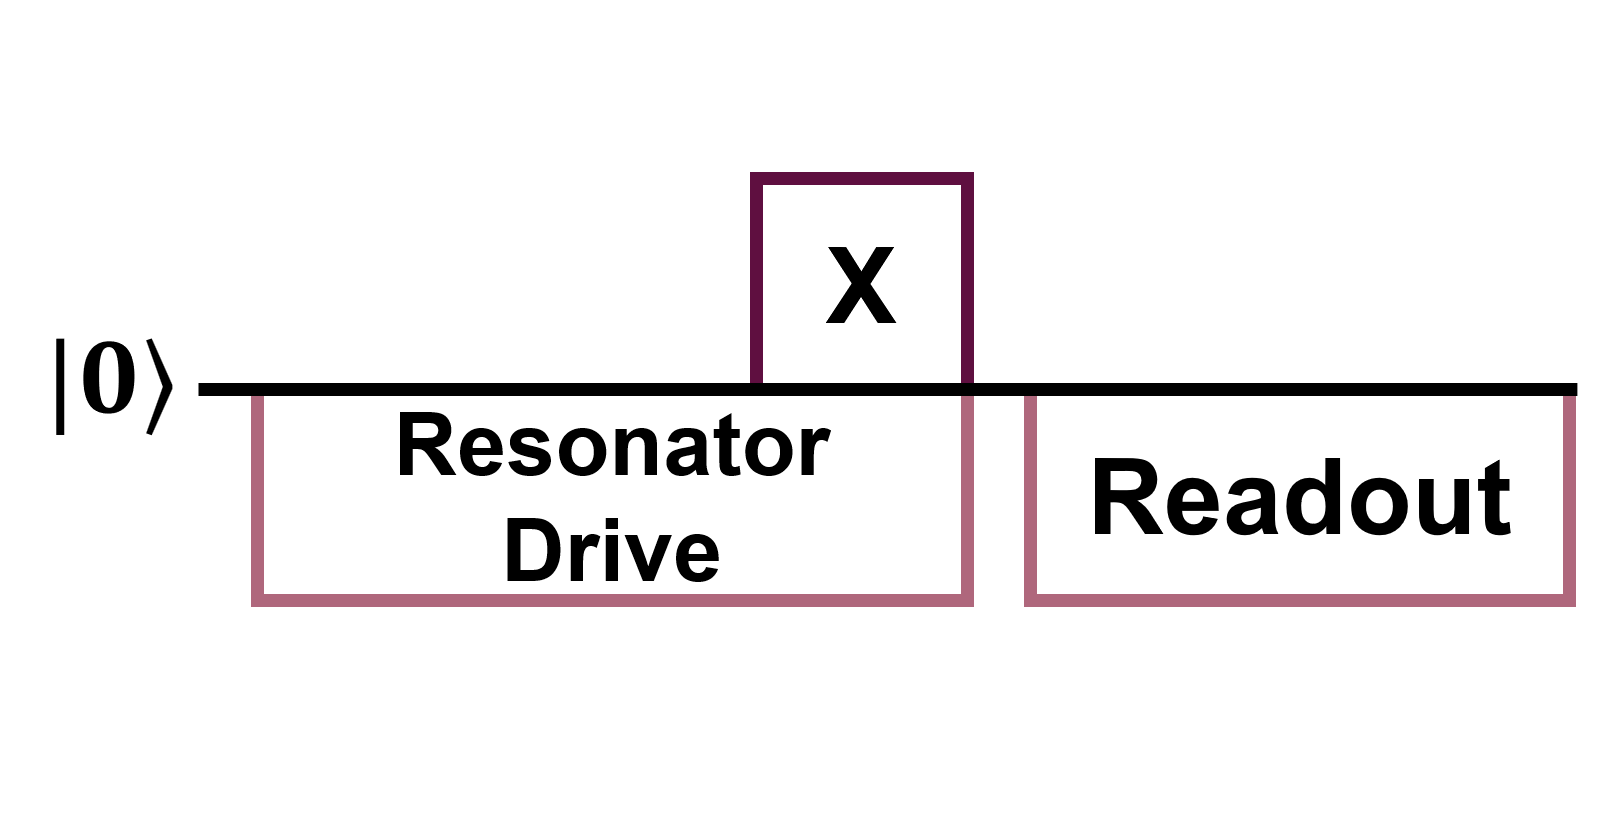
\includegraphics{Figs/circuits/photon_counting.png}
    \caption{An illustration of the photon counting experiment. A pulse is applied with the amplitude of the typical readout pulse. When the steady state is reached an X-gate with a a given frequency is applied. A typical readout is performed thereafter to see if the qubit changed state.}
    \label{fig:photon_counting_circuit}
\end{marginfigure}

\begin{figure*}[h]
    % \begin{minipage}{0.60\linewidth}
    \centering
    % 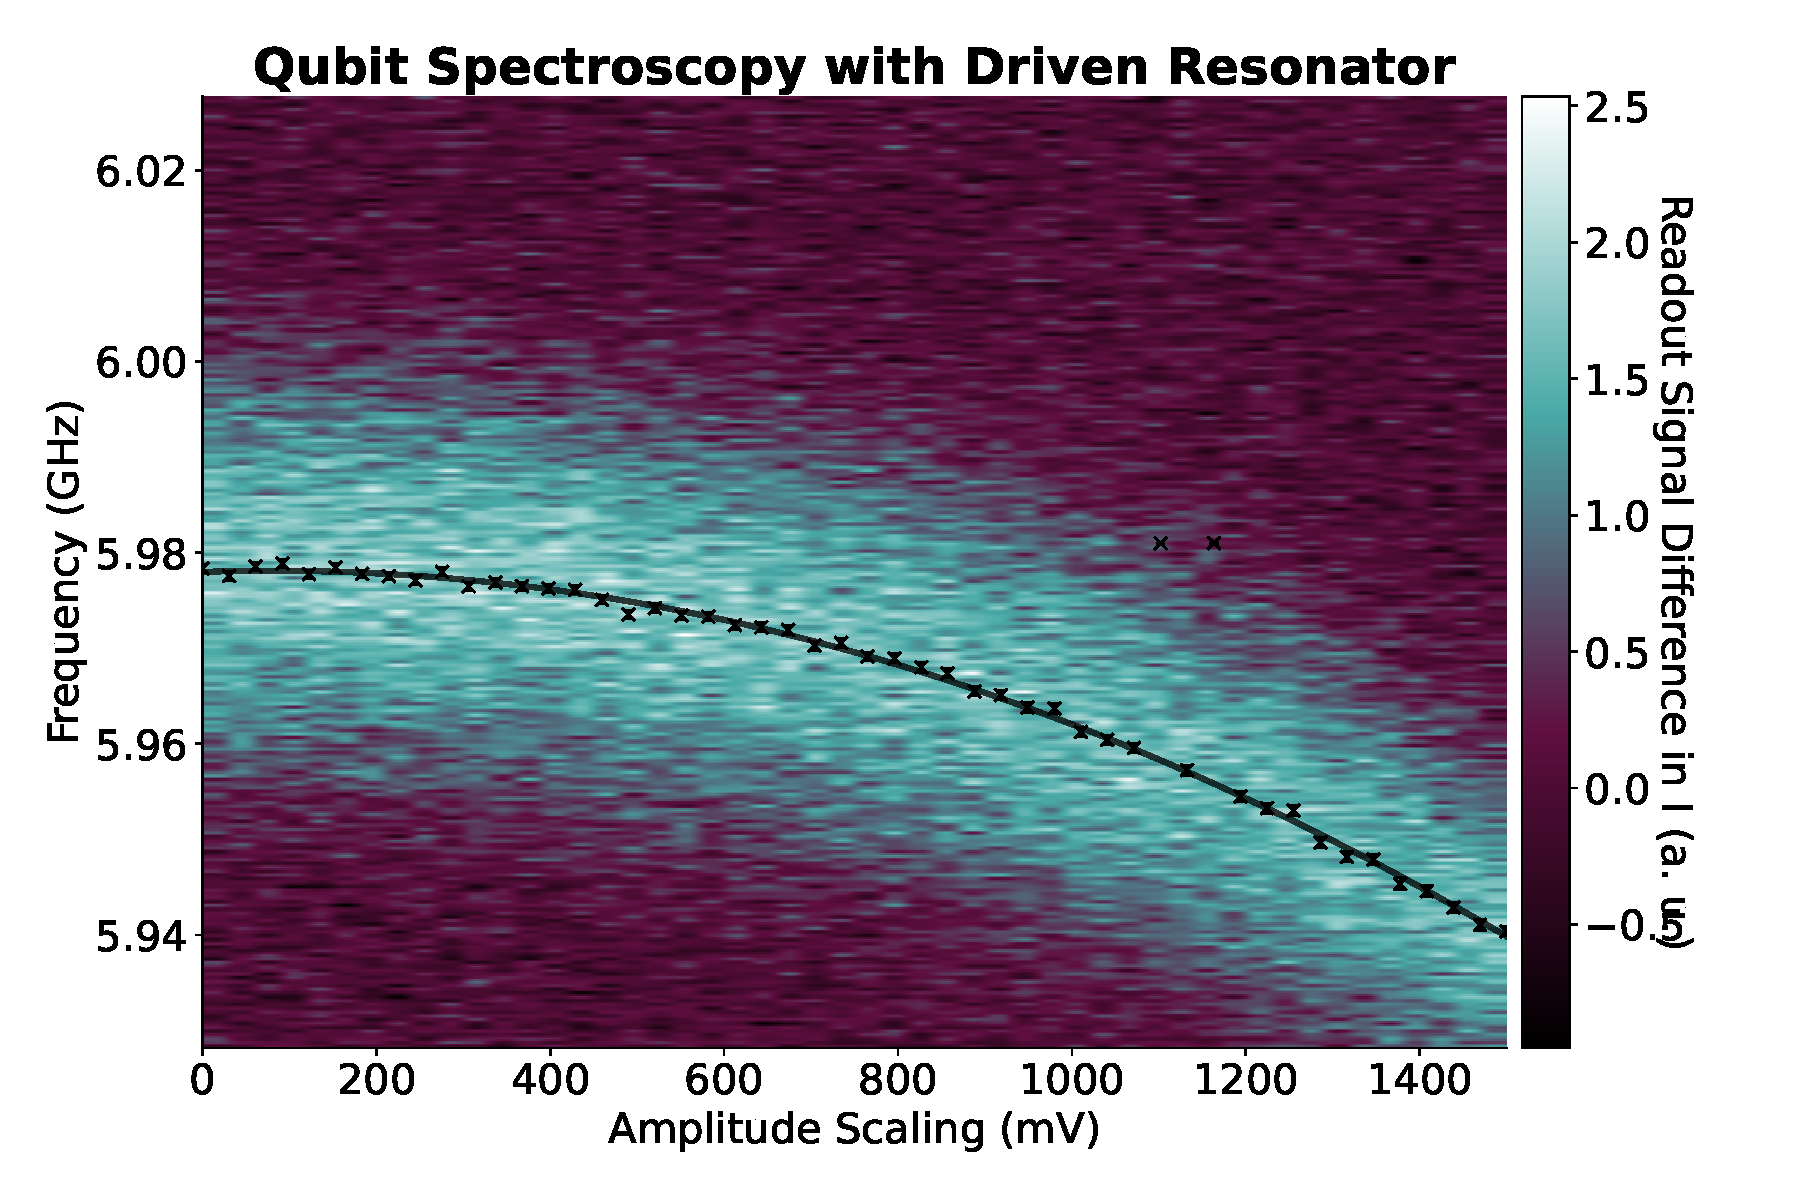
\includegraphics[width = \linewidth]{Calibrations/Figures/Qubit Spectroscopy with Driven Resonator.pdf}
    % \end{minipage}
    % \begin{minipage}{0.40\linewidth}
        % \centering
    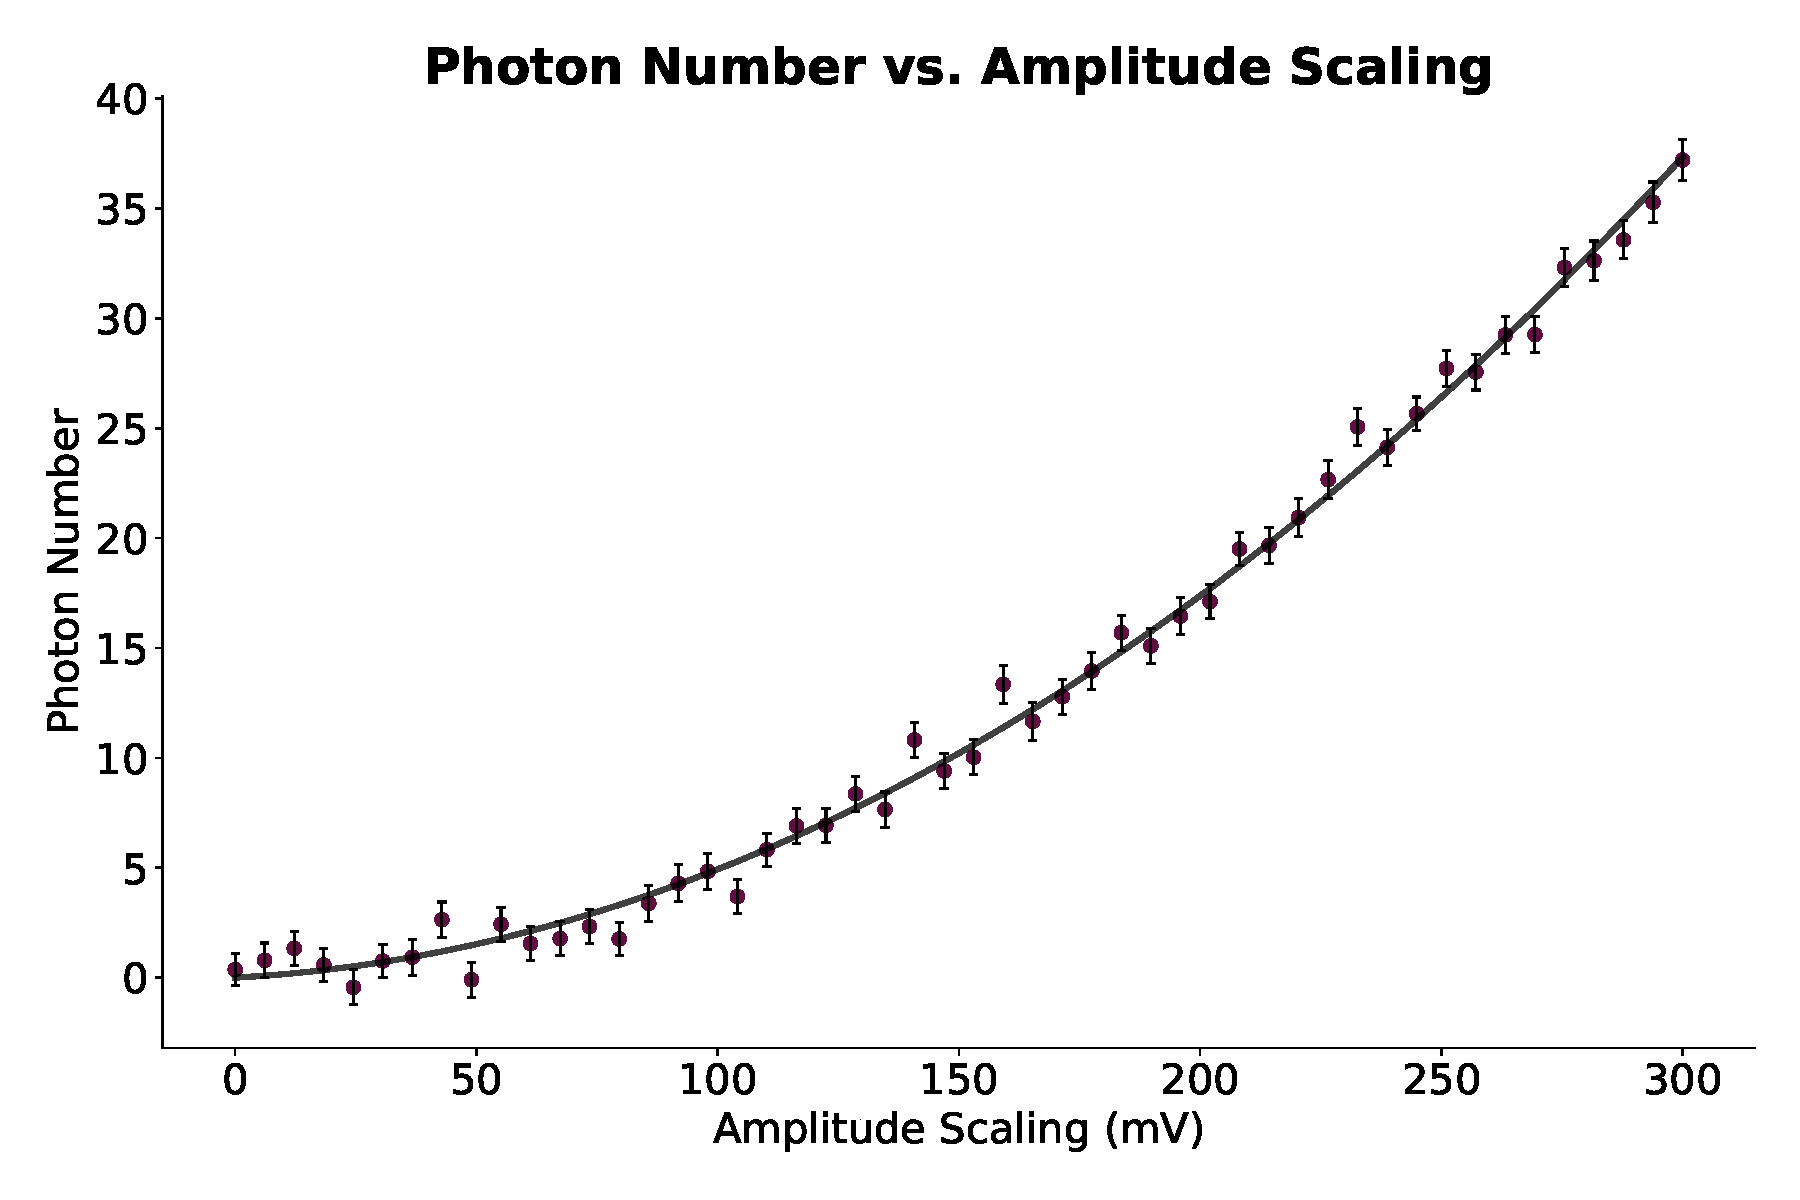
\includegraphics[width = \linewidth]{Calibrations/Figures/photon_number.pdf}
    % \end{minipage}
    \caption{Scan of readout-pulse-amplitude and the frequency of qubit-pulse in the left plot. The right shown the calculated mean photon number.}
    \label{fig:calibration_photon_counting_scan}
\end{figure*}
From this analysis, we extract the mean photon number as:
\begin{equation}
    \Bar{n}_{\text{ss}} = 21 \pm 1
\end{equation}

Which we can use to extract the driving strength seen by the resonator from equation \ref{eq:steady_state_amplitude}
\begin{equation}
    \epsilon = \Bar{n} \sqrt{\left(\frac{\kappa}{2}\right)^2 + (\chi)^2} = 6.4 \text{ MHz}
\end{equation}
When driving the resonator at its frequency $f_r$.


% If we now fit a Lorentzian curve over the frequencies for each amplitude and divide with the dispersive shift from equation \ref{eq:dispersive_shift}, we can obtain the relation between steady state photon number and the readout amplitude. This fit can be seen in figure \ref{fig:calibration_amplitude_photon_number}. \textit{By further extracting the $|I+iQ|$ value at each amplitude in a regular readout, we can also get a linear equation. By combining the two slopes we can scale the voltage values to resonator photon count. This also allows us, to find the amplitude $\epsilon$ experienced in the drive, which is a more complex combination of physical parameters on the chip as well as the applied feed line voltage.}

% % \begin{figure}
% %     \centering
% %     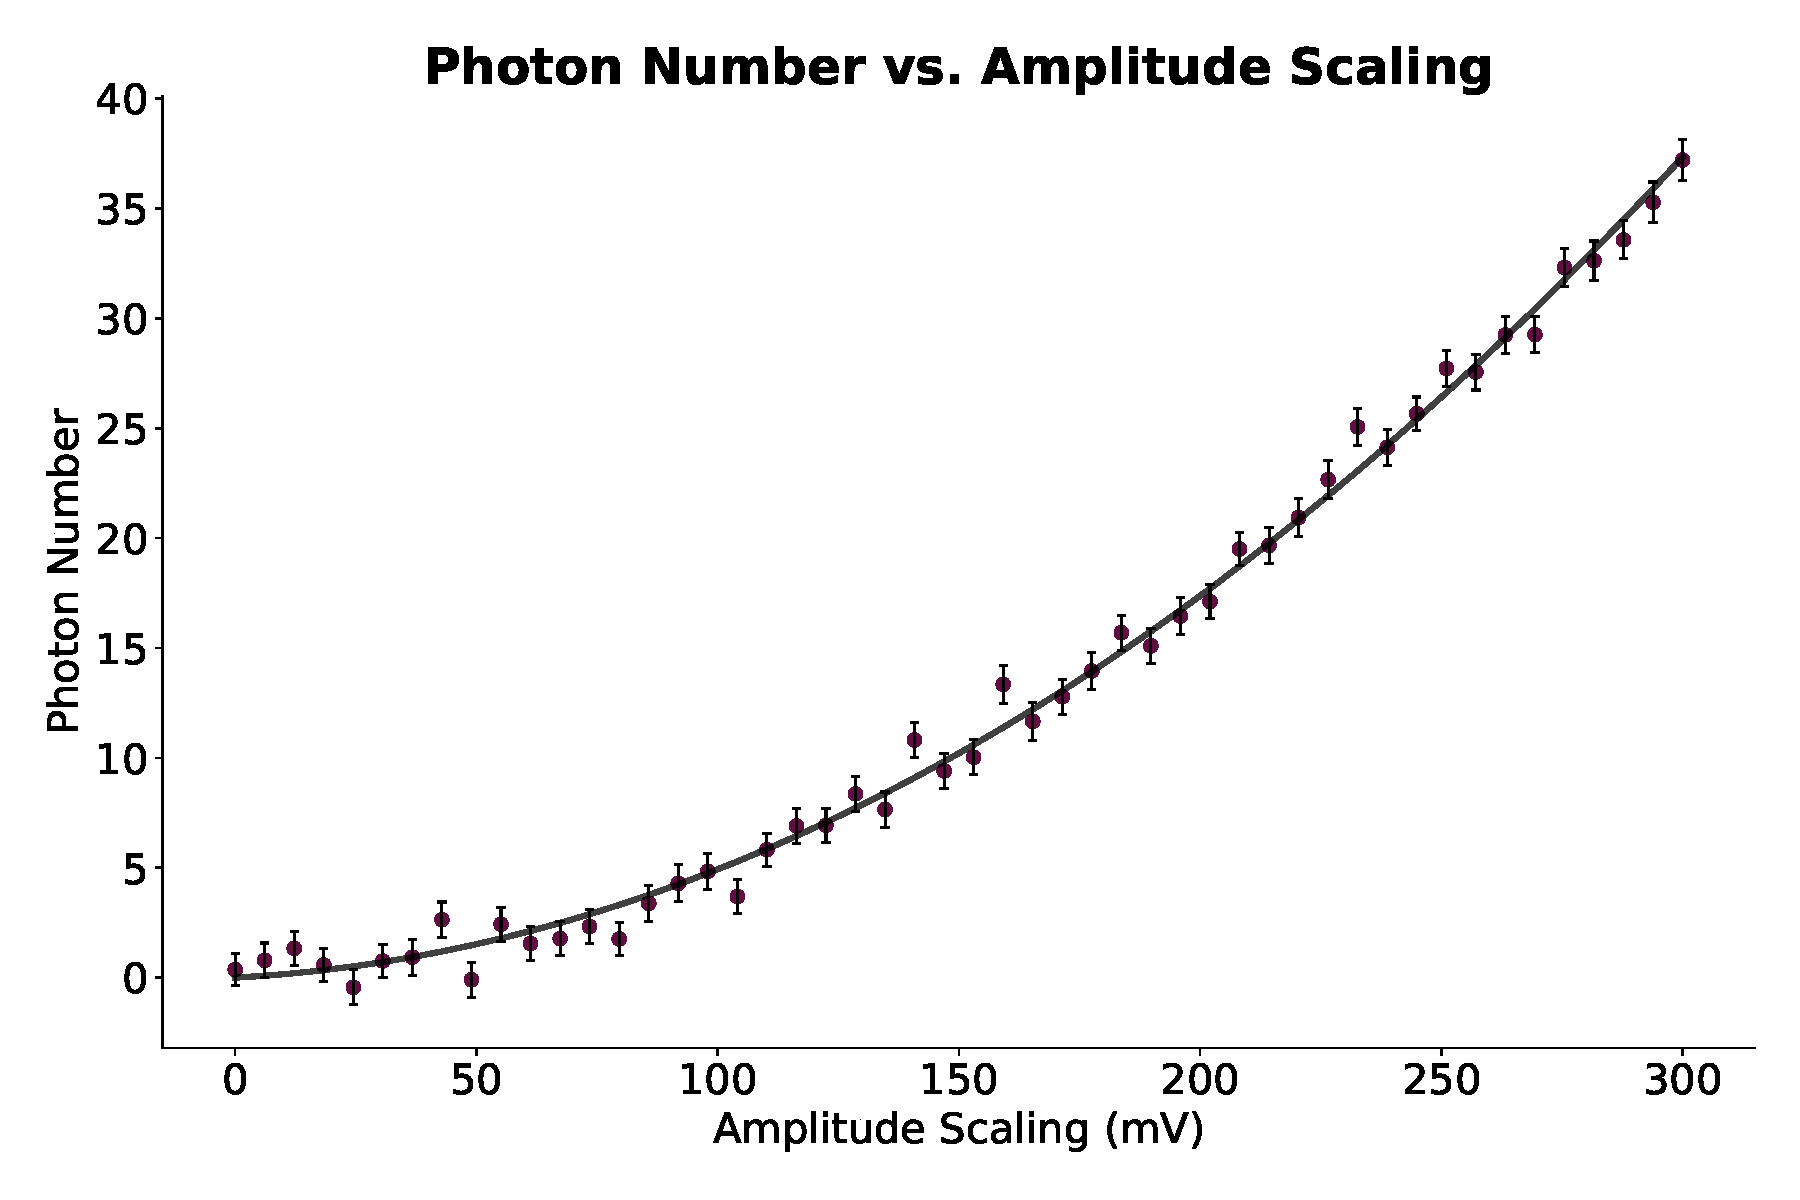
\includegraphics[]{Calibrations/Figures/photon_number.pdf}
% %     \caption{Caption}
% %     \label{fig:calibration_amplitude_photon_number}
% % \end{figure}

% By doing the analysis, we can fit a polynomial to get the form of the curve. This allows us to estimate the value at $100\%$ of the actual readout amplitude. This allows us to estimate the mean photon number of the readout end of the readout to be:


% One big challenge still stands, how do we map the axis to each other?  


% Considering the dispersive hamiltonian of the qubit-resonator-system, Eq. \ref{eq:two_level_qubit_dispersive}, we have above primarily considered the shift of resonator frequency depending on the qubit state, but just moving the parenthesis to represent it in the form:
% \begin{equation}
%     H = \Tilde{\omega}_r a^\dagger a  + \left(\frac12 \Tilde{\omega}_{01} + \chi a^\dagger a\right)  \sigma_z
% \end{equation}
% making it apparent that while the qubit state moves the resonator, the opposite is also true. Since the qubit frequency moves with $\chi$ for each photon in the resonator, we 




% The protocol is carried out in the following way:
% \begin{itemize}
%     \item Drive the resonator at a given amplitude to fill it with photons.
%     \item When the resonator is in its steady state apply an X-gate with a given frequency.
%     \item Perform a regular readout
% \end{itemize}
% By sweeping over amplitude and X-gate frequency, one can find the resonance frequency at every amplitude. Since the resonance frequency is related to the qubit \\

% % \begin{marginfigure}[- 5 cm]
% %     \centering
% %     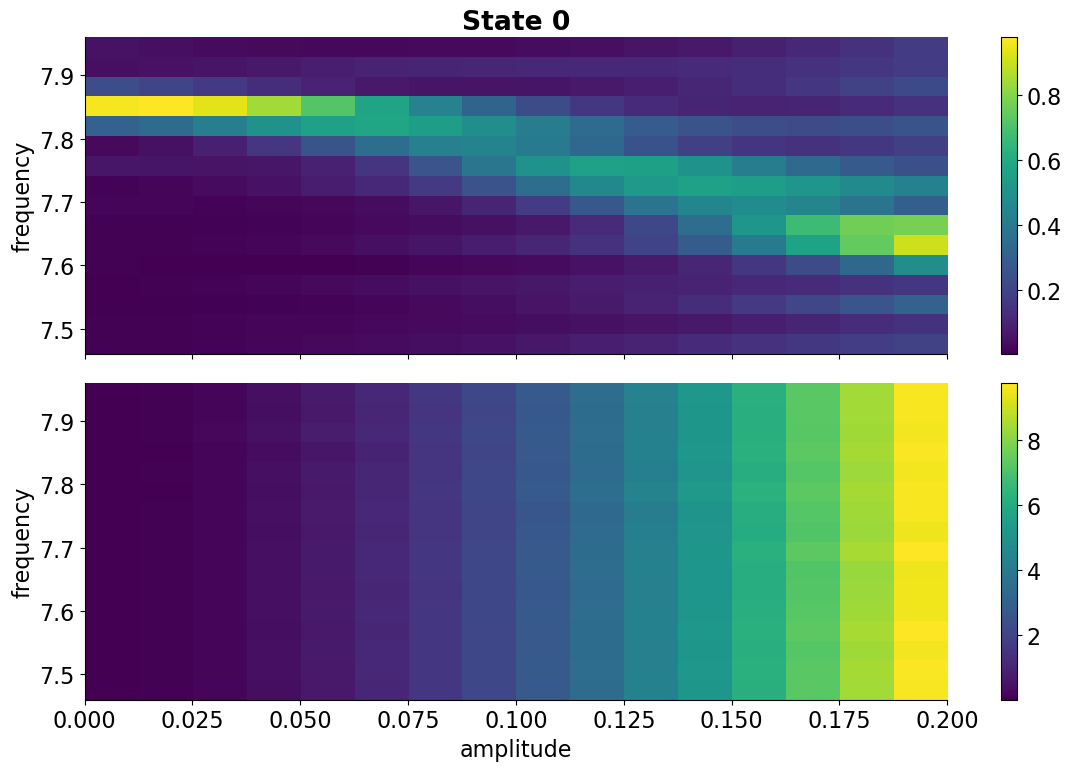
\includegraphics[width = 1.3 \textwidth]{tex/fig_for_text/section_6/photon_number_calibration.png}
% %     \caption{Simulation of photon number calibration protocol.  }
% %     \label{fig:photon_number_calibration}
% % \end{marginfigure}

% \noindent
% \textbf{We need the following Data}:
% \begin{itemize}
%     \item First calibrate the double dip and find the dispersive shift from above
%     \item For the $\ket{0}$, we should drive the resonator at the resonator frequency and measure the $|I + iQ|$
%     \item For the $\ket{1}$, we fill the resonator with photons and apply an x-gate with a given frequency. Scan over this frequency to find the resonance frequency as a function of amplitude $\to |I + iQ|$ measured above
%     \item We should repeat this experiment where we apply another readout frequency to the most optimal (probably in between the two peaks). 
% \end{itemize}

\section{System Parameters}
Lastly, the dynamics of the combined system are subject to two additional outside forces: the temperature $\tau$ and the efficiency of the amplification chain $\eta$.


\subsection{Temperature and $T_1$ Calibration in Continuous Time}\label{sec:continuous_calibratino}
In section \ref{sec:theory_t1}, we covered how $T_1$ and $\tau$ has effects on the dynamics and equilibrium positions of the density matrix. In this section, we have developed a method (very similar to the $T_1$ calibration from section \ref{sec:calibration_t1}) that uses continuous time-traces to determine these parameters. It should be noted that the experiment run here is made a few months before the other calibration schemes at a time where $T_1$ was significantly higher. The temperature is however still representative of the state of the qubit when the readout experiment in chapter \ref{chap:readout} was made.



In this experiment, we will do a long continuous readout pulse of the resonator. By splitting it up into small chunks, we will see the state of the qubit at that given time. If we repeat this experiment $n$ times, then we can estimate $\rho_{00}(t)$ and $\rho_{11}(t)$ at a given time during the readout. Since the readout primarily adds dephasing of the qubit, this should not influence the diagonal components of the density matrix. The time dependent elements of the density matrix can now be fitted with the equations derived in section \ref{sec:theory_t1}. The data from a thousand trajectories of $50 \text{ µs}$ classified by demodulating sections of $1 \text{ µs}$ is shown in figure \ref{fig:continous_calibration_decays} and the distributions and classifications from demodulating the first microsecond is displayed in figure \ref{fig:IQ_distribution_temp}. By doing $1 \text{ µs}$ intervals, we significantly reduce the overlap between the two distributions, such that it can be neglected in the steady state count.
% \begin{marginfigure}
%     \centering
%     \missingfigure{T1 circuit}
%     \caption{Caption}
%     \label{fig:inmeasurementt1circuit}
% \end{marginfigure}
% Performing the circuit described in figure \ref{fig:inmeasurementt1circuit} multiple times. We modulated the signal and course grained it in $10 \text{ ns}$ intervals to reduce data size. By doing $1 \text{ µs}$ summations and classifying\footnote{Classification schemes can be made by taking a subsample and drawing a thresh hold line with data from the first $1 \text{ µs}$ where the distribution most close resembles the initialization.} each individually, we can see the distribution of $\ket{0}$ and $\ket{1}$ over the entire readout duration. In an example with $50 \text{ µs}$ long readout the following distributions were found for qubit initialized in the ground and first excited state respectively see figure \ref{fig:continous_calibration_decays}. 
\begin{figure}
    \centering
    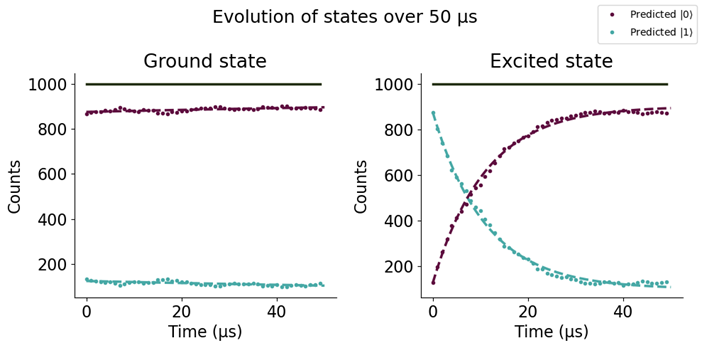
\includegraphics{Figs/calibrations/contiuous/decays.png}
    \caption{The dynamics of our qubit system from $50 \text{ µs}$ readout split into $1 \text{ µs}$ pieces which are all classified.}
    \label{fig:continous_calibration_decays}
\end{figure}
% \begin{margintable}[3 cm]
%     \centering
%     \caption{Table of results from experiment}
%     \begin{tabular}{c|cc}
%         & Ground State & Excited state \\

\begin{marginfigure}
    \centering
    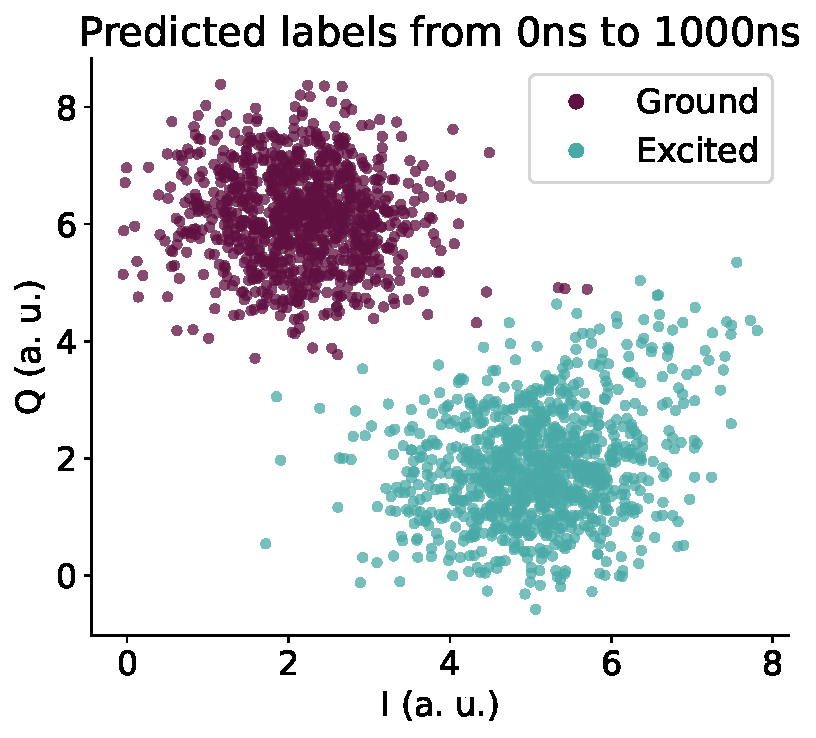
\includegraphics{projects/in_measurement_calibration/Distributions_long_pulse.pdf}
    \caption{The IQ distribution of points from a 1 microsecond demodulation window. The two distributions are well separated, so we expect no overlap.}
    \label{fig:IQ_distribution_temp}
\end{marginfigure}
%         \hline
%         $\rho(\infty)$&$0.951 \pm 0.254$&$0.099 \pm 0.004$ \\
%         $\rho(0)$&$0.875 \pm 0.003$&$0.124 \pm 0.008$\\
%         $T_1$ &$(159 \pm 615) \text{ µs}$&$(11.1 \pm 0.3)  \text{ µs}$\\
%     \end{tabular}
%     \label{tab:continous_calibration_decays_results}
% \end{margintable}
From the results of the fitted parameters (see table \ref{tab:continous_calibration_decays_results}), we can extract the decay time, the initial fraction and the steady state fraction of occupancy in the excited state $\ket{1}$. We initialized both in $\ket{1}$ and $\ket{0}$, but since the state ground state initialization is already in steady state, we will not trust the fit parameters. While the idea of the method originally was to determine $T_1$ with a fast scheme, the important aspect for this thesis is to extract the temperature from the steady state fraction. We find the temperature from the Boltzmann factor in the steady state:
\begin{fullwidth}
\begin{equation}
    \frac{\rho_{00}(t=\infty)}{\rho_{11}(t=\infty)} = e^{(E_1 - E_0) / k_b \tau} \Rightarrow \tau = - \frac{\hbar \omega_{01}}{k_b} / \log\left(\frac{\rho_{00}(t=\infty)}{\rho_{11}(t=\infty)}\right)  =  (0.13 \pm 0.04) \text{ K}
\end{equation}
\end{fullwidth}
One might compare the temperature of the superconducting qubit with the temperature of the cryostat of around 30 mK. The difference is suspected to come from electronic heating and other sources of microwaves leaking out into the material. The first run of this analysis gave $\tau =  147.5 \text{ mK}$ which is the value used in simulation. This is however well within the confidence interval.


\subsection{Readout Efficiency}\label{sec:readout_efficiency}
The amplification chain from the resonator signal and up to room-temperature and digitization is by no means lossless. Each amplification and thermalization step adds noise to the coherent state of the resonator state which we are trying to measure. This ultimately gives us a state which is severely blurred if we compare it to the crisp coherent states with widths of only $1/2$. In this subsection, we will estimate the efficiency parameter $\eta$. We will follow the method developed by Bultink et al. \cite{bultink_general_2018} where they perform this calibration in general for the whole amplification chain.

The general idea can be found in the inefficient stochastic master equation (see section \ref{sec:sme_inefficient}). Here the backaction term is applied no matter the efficiency we measure with, such that the qubit is dephased. By comparing the amount of extracted information with the amount of dephasing, we can estimate the efficiency. %In section \ref{sec:qubit_backaction}, we mentioned that measuring the resonator adds a back action to the qubit which takes the form of a dephasing Lindbladian. Furthermore, the signal measured will be of the coherent states associated with $\alpha_0$ and $\alpha_1$ and be divided by the noise in the system.

To use this method, one must first create a readout pulse with a signal that is zero at start and end: $S(t = 0) = S(t = T) = 0$. To limit decoherence during the readout, one would choose a short pulse and readout during a cooldown of the resonator for $\approx 5 / \kappa$.\footnote{One can optimzie this further by applying a stimulated depopulation pulse.} The shape and resonator signal in pulse is shown in figure \ref{fig:efficiency_pulse_shape}. With this pulse, the method now consists of two parts:

% \vspace{2 cm}
% The amplification chain from the qubit and resonator up to our digitization of the signal is by no means lossless. As mentioned in section \ref{sec: Amplifiers}\todo{Write section about amplifiers} there is a lower bound on the amount of noise added by an amplification. But in addition, the signal sees multiple amplification and thermalization at different stages ultimately giving us a much noisier signal than what is actually extracted from the qubit. To include this effect in our simulation and just to benchmark the amplification chain we will extract the quantum efficiency, $\eta$ by a method presented in \cite{bultink},\todo{Cite properly the Bultink et al. article} where the backaction of the qubit is compared to the Signal to Noise Ratio of the output signal. 

\begin{marginfigure}
    \centering
    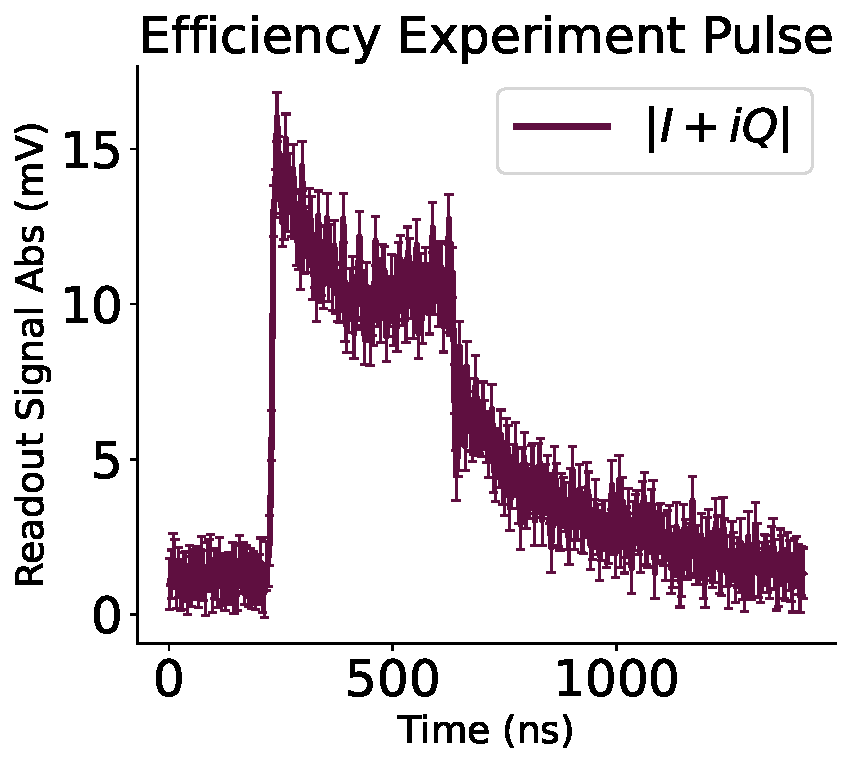
\includegraphics{Calibrations/Figures/Efficiency Experiment Pulse.pdf}
    \caption{The signal in the resonator during the readout pulse used for the efficiency calibration.}
    \label{fig:efficiency_pulse_shape}
\end{marginfigure}

\begin{enumerate}
    \item Determine how the SNR changes when we increase the readout amplitude. With a signal starting and ending at 0, this should follow a linear relation: $\text{SNR}(\epsilon) = a \epsilon$.
    \item Investigate the backaction of the readout on the qubit. After a pulse, the coherence is related to the readout amplitude by the gaussian relation $|\rho_{01}(T, \epsilon)| = |\rho_{01}(T, 0)|e^{-\epsilon^2/2\sigma^2}$
\end{enumerate}
From these parameters, the readout efficiency can then be calculated as \cite{bultink_general_2018}:
\begin{equation}
    \eta = a^2\sigma^2
\end{equation}
where our equation deviates from the one in \cite{bultink_general_2018} by a factor $2$, since they define $\SNR$ with respect to the variance of a single trajectory\footnote{assuming that the trajetory for the ground and excited state has the same variance.}, whereas we combine the two $\text{Var} = \text{Var}_{\ket{0}} + \text{Var}_{\ket{0}}$ reducing the SNR with $1/\sqrt{2}$ compared to their definition.

\paragraph{Amplitude Dependence of SNR - }
To determine the Signal to Noise ratio from the readout pulse, we do a readout experiment like the one in chapter \ref{chap:readout}: by initializing the qubit in $\ket{0}$ and then performing an $X$-gate to every other initialization before reading it out, one can see determine the separation between $\ket{0}$ and $\ket{1}$. We make sure to use optimal weights, to make sure all the available information is used.

% \begin{marginfigure}
%     \centering
%     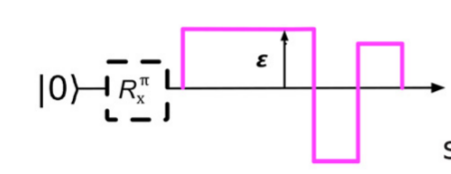
\includegraphics{Figs/calibrations/efficiency/experiment_circuit_SNR.png}
%     \caption{Circuit for experiment}
%     \label{fig:efficiency_SNR_experiment}
% \end{marginfigure}

By repeating the experiment for drives with different fractions of the readout amplitude $\epsilon$ and calculating the SNR from the measurement distributions, we obtain the results in the left panel of figure \ref{fig:effiiency_results_SNR}. To the right, the histogram is shown for the $I$ for $\epsilon / 4$. The SNR is calculated by taking $\sqrt{\SNR_I^2 + \SNR_Q^2}$. Fitting a linear equation to the results, we obtain $a = (2.43 \pm 0.15) / \epsilon$. 

\begin{figure}
    \raggedleft
    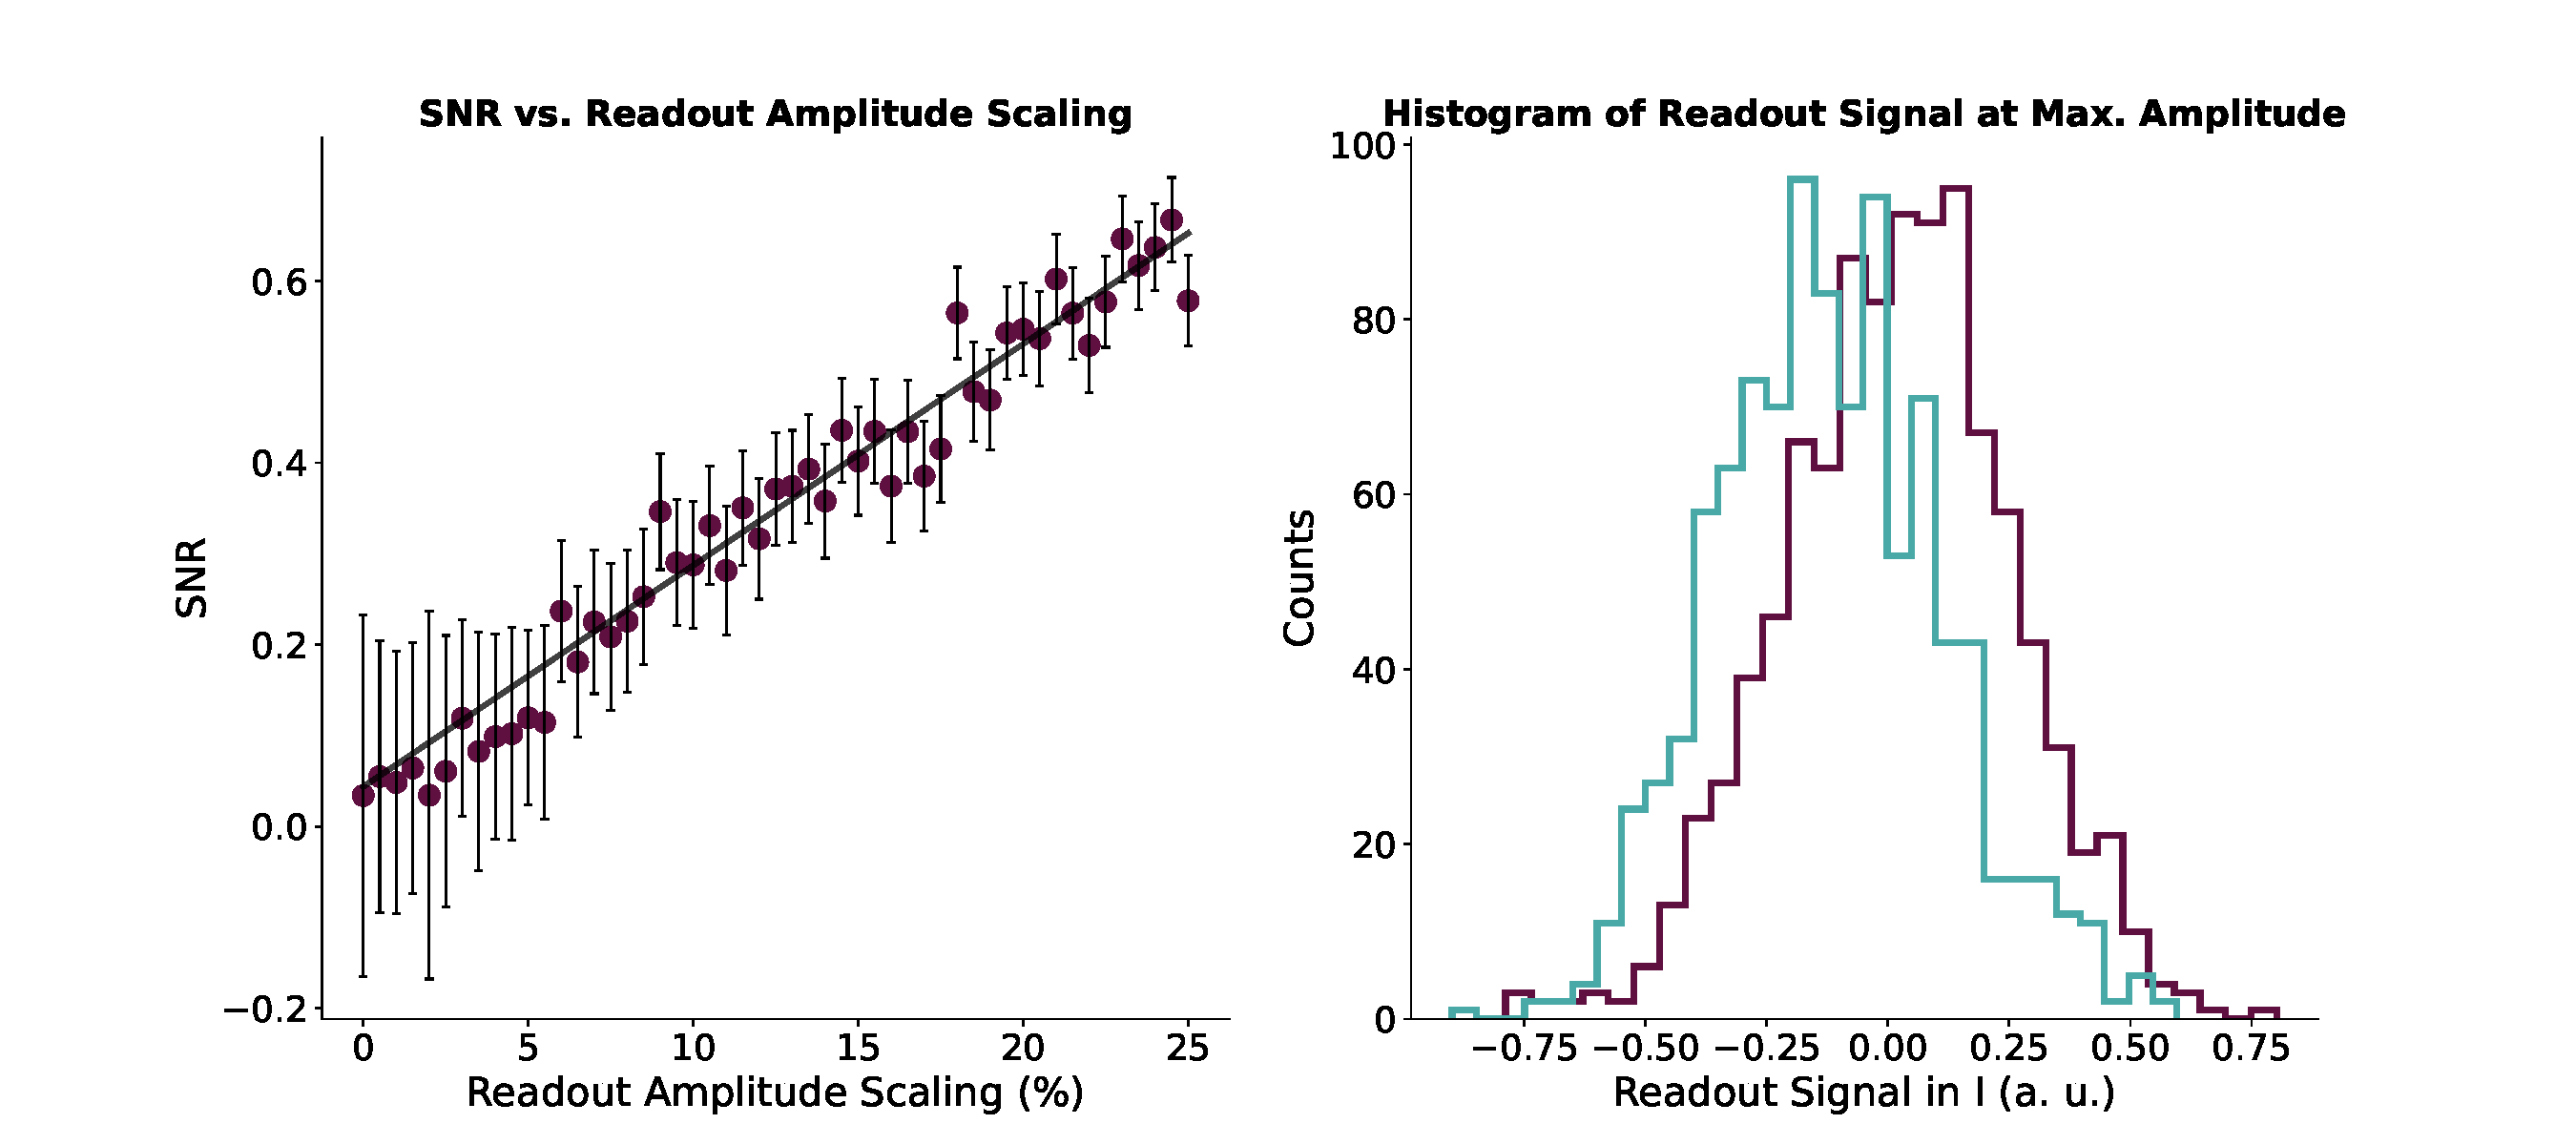
\includegraphics[width = 1.0 \linewidth]{Calibrations/Figures/SNR_vs_amplitude.pdf}
    \caption{Figure showing the experiment for extracting SNR as a function of readout amplitude. An example at the highest amplitude is shown, where the two distributions are separated. The SNR is extracted as $\text{SNR}^2 = \expval{S_{\ket{0}} - S_{\ket{1}}}^2/\left(\expval{S^2_{\ket{0}}} +\expval{S^2_{\ket{1}}}\right)$. The other figure displays the result of this analysis for all values of $\epsilon$ as well as a linear fit applied to it.}
    \label{fig:effiiency_results_SNR}
\end{figure}



\paragraph{Dephasing from Readout Pulse}
For finding the relation between the amplitude and dephasing, the qubit is initialized in $\ket{0}$ and a $R^x_{\pi/2}$ pulse is performed to send the qubit into $\frac{1}{\sqrt{2}}\left(\ket{0} + i\ket{1}\right)$. With the pulse in this state, the density matrix will be:
\begin{equation}
    \rho(t=0) = \frac12 \begin{pmatrix}1 & -i \\ i & 1\end{pmatrix}
\end{equation}
the readout drive will now be applied\footnote{Just as pulse because we're not interested in the signal}. During the readout signal the off-diagonal elements will be reduced by two factors: inherent dephasing by $T_2$-processes and qubit back action by the signal. To determine the amount of dephasing, we will perform a $\pi/2$ rotation around an axis along the $\phi$ angle in the x-y-plane before reading out the signal. The entire sequence is illustrated in figure \ref{fig:efficiency_dephasing_experiment}.

\begin{marginfigure}[-6 cm]
    \centering
    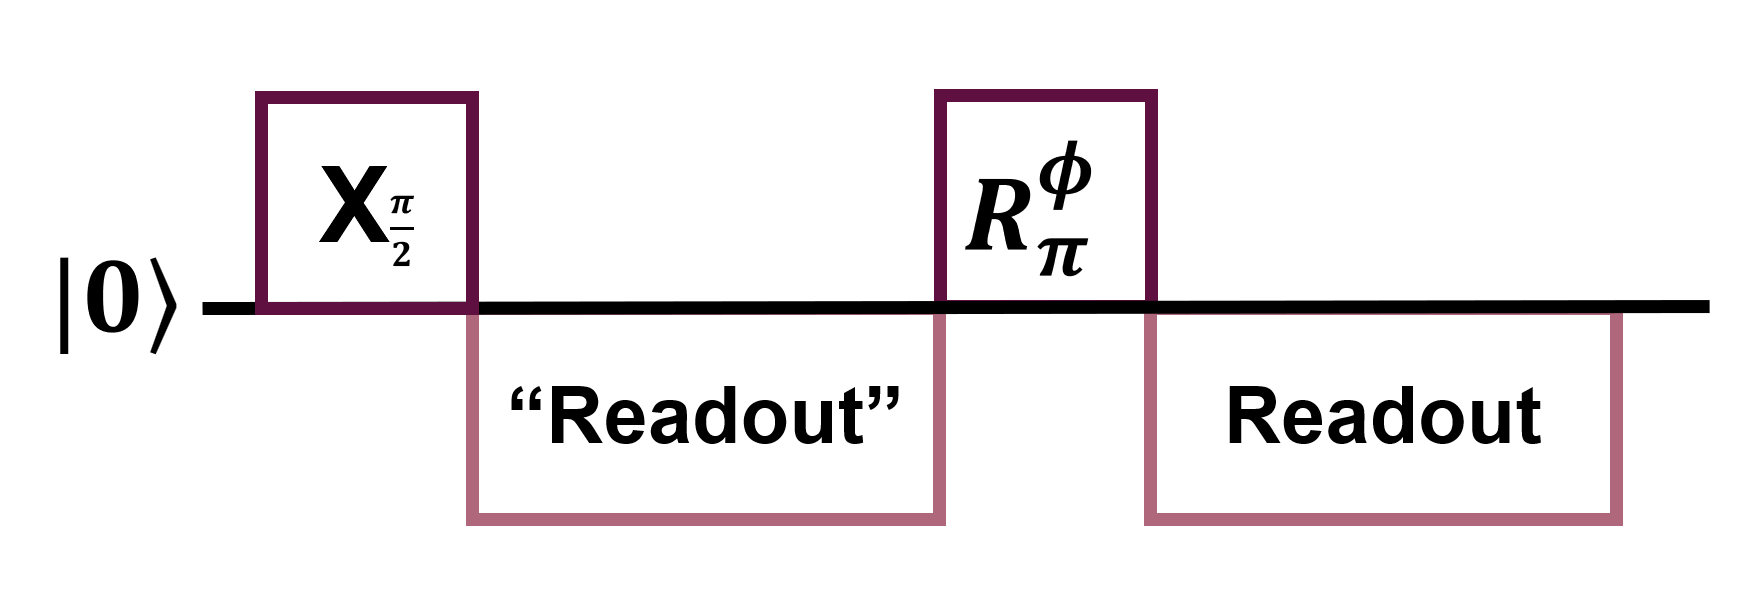
\includegraphics[]{Figs/circuits/dephasing.png}
    \caption{The dephasing experiment circuit. First the qubit is rotated $\pi/2$ around the X-axis, where after it is subject to the readout pulse without demodulating and saving the signal. Now the qubit is rotated $\pi$ around a vector $\phi$ in the $x-y-$plane and finally readout.}
    \label{fig:efficiency_dephasing_experiment}
\end{marginfigure}
\begin{figure*}
    \centering
    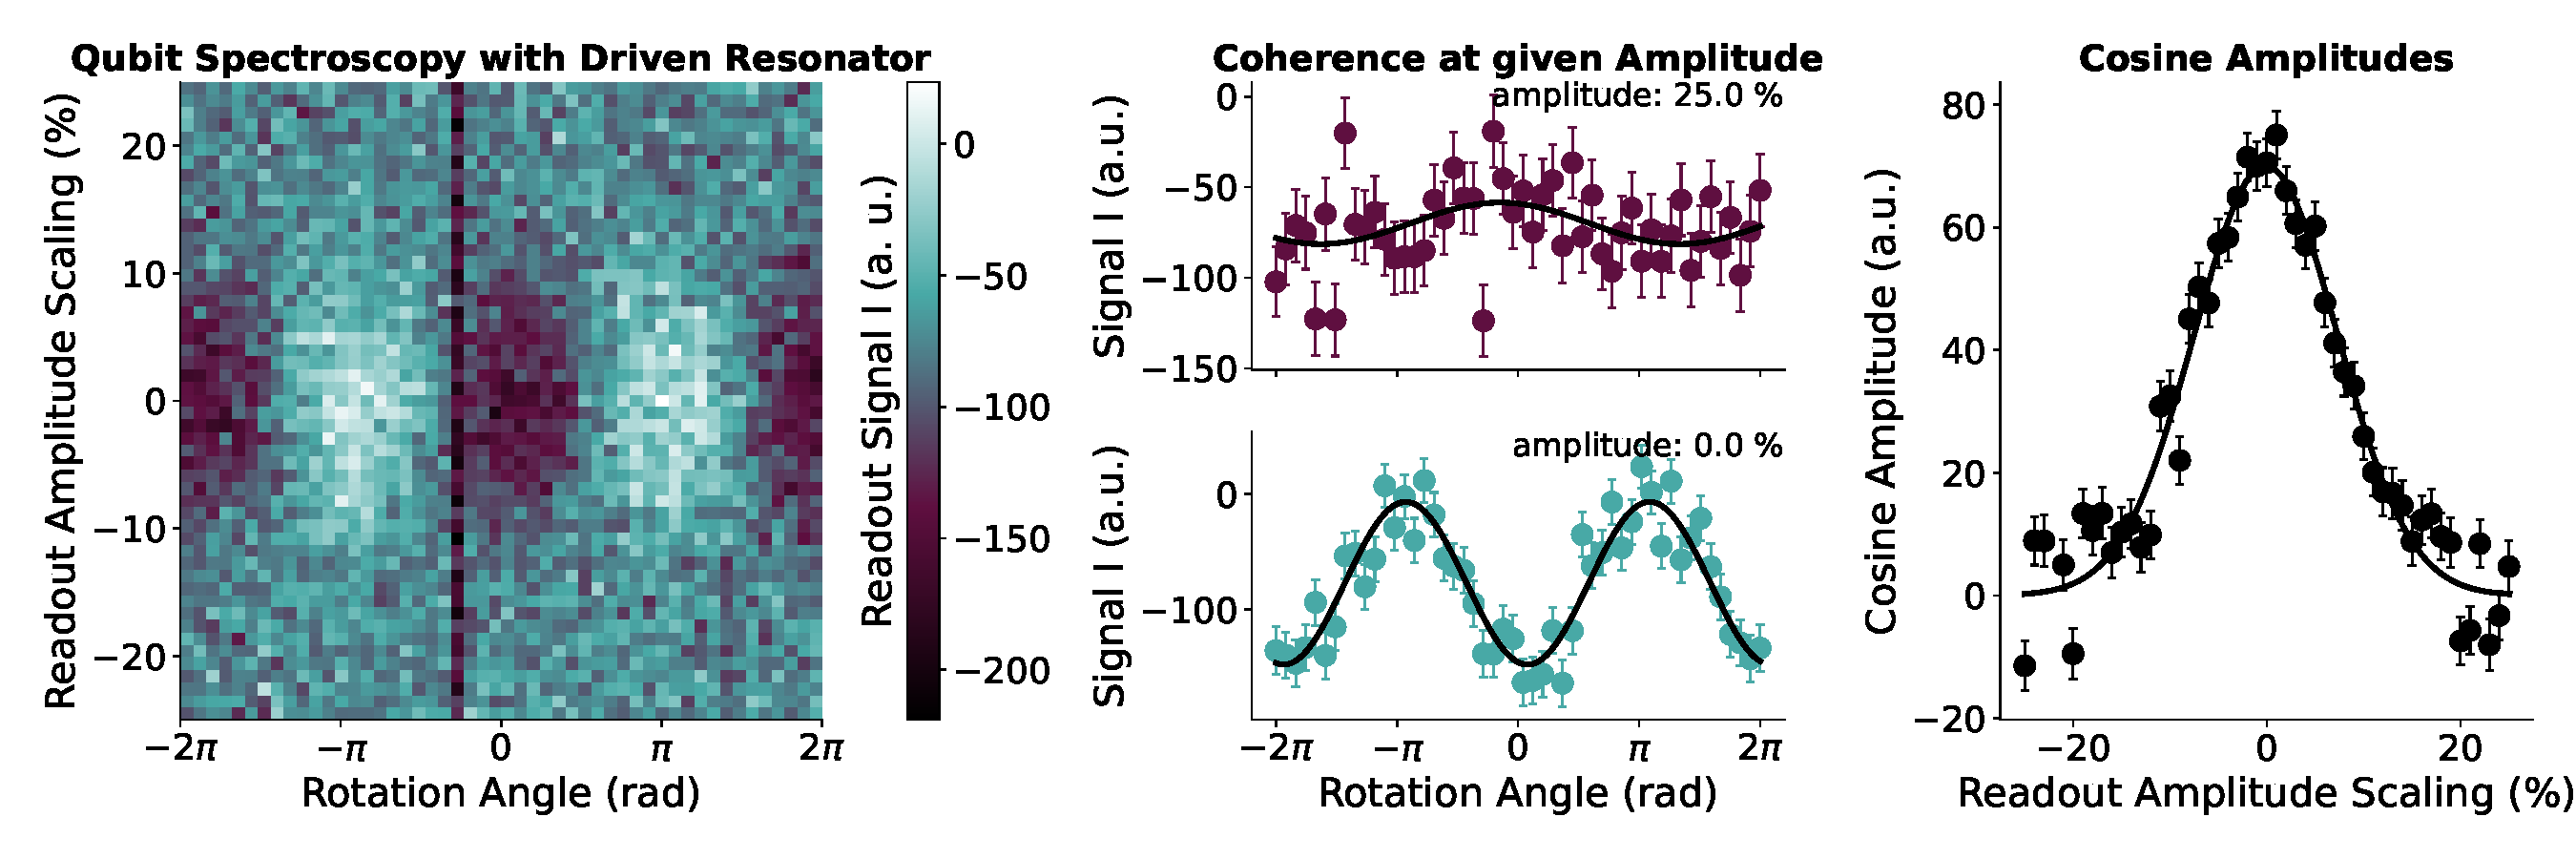
\includegraphics{Calibrations/Figures/dephasing_by_measurement.pdf}
    \caption{Results from the dephasing experiment. The 2D scan is shown along with the cosine-way for amplitude $\epsilon = 0$ and $\epsilon = \epsilon_{max}$. Fitting the cosine function and plotting the amplitude as function of the readout amplitude gives the last figure, where they are are fitted by a Gaussian distribution.}
    \label{fig:efficiency_dephasing_result}
\end{figure*}

By comparing the readout signal for different angles of $\phi$, we expect a cosine shape: $\expval{\sigma_z} = 2 |\rho_{01}(t= T)| \cos(\phi+\phi_0)$. Repeating this for different fractions of the readout amplitude, we can fit a Gaussian distribution to determine $\sigma$. Here the $T_2$ dephasing will just contribute to an overall dephasing, which will be constant throughout all the experiment. However,  this does not affect the width of the Gaussian, which we are interested in. The outcome of the distributions can be seen in figure \ref{fig:efficiency_dephasing_result} where we find a value for $\sigma = (7.42 \pm 0.17)\; 10^{-2} \; \epsilon$.
% And repeating for different readout amplitudes the dephasing due to back action can be separated from the one due to $T_2$-dephasing which only has an effect of the amplitude. The results of the experiment can be seen in figure \ref{fig:efficiency_dephasing_experiment}, where the parameter from the important parameter for the Gaussian fit is the standard deviation: $\sigma = (7.42 \pm 0.17) \times 10^{-2} \; \epsilon$. \marginnote{Write the $\chi^2$ and $p-val$ for the fit in the marginnote.}

We note that there is some problem along a specific rotation axis. When using the OPX, there is sometimes an accumulation of phases, which can give specific errors, so we will here ignore data along that axis. The phase and frequency of the cosine shape is fitted in the case where the amplitude of the applied readout pulse i 0. And is kept fixed for all other amplitudes.

\paragraph{Calculating the Efficiency}
In the last two experiment we have extracted $a$ and $\sigma$. By combining them, we can find the efficiency of the readout chain:
\begin{equation}
    \eta = a^2\sigma^2 = (3.3 \pm 1.2) \% 
\end{equation}




% \paragraph{Interleaved Experiment *}\todo{Do analysis} Since the $T_1$ can vary a lot over even small time periods, we also perform and interleaved version of the old and new experiment. This will also allow us to see if there is a different decay inside and outside of the measurement. In this experiment the previous one is carried out again but this time we will include a sweep over the waiting time before reading out for the same pulse length. We can now compare the in-measurement $T_1$ values from the fit within the same pulse with the ones across the waiting time. Given that we see a constant offset $T_1^{meas} = T_1^{wait} + \delta t$ this will show up in this experiment,

% \begin{figure*}
%     \centering
%     \missingfigure{Analysis of interleaved experiment}
%     \caption{Caption}
%     \label{fig:enter-label}
% \end{figure*}

% Comments on results... 


\FloatBarrier
\section{Overview of Device Parameters}\label{sec:overview_section}
In this chapter, we have calibrated the necessary values of the qubit, resonator and system to be able to simulate the quantum system. The parameters are summarized in table \ref{tab:qubit_calibration}. In determining some parameters and uncertainities, the model was not a good fit for our data. These parameters are marked with a star * to illustrate that not much weight should be contributed to the listed value.


\begin{table}[h]
\centering
\caption{The outcome of calibrating the qubit with the methods presented in this chapter. A star * illustrates that a value comes from a modified fit or that the uncertainty is taken from a fit with a very high or very low reduced $\chi^2$. }
\begin{tabular}{lr|rrr}
\hline
\textbf{Qubit}                &          & value & error  & unit \\ \hline
Frequency                     & $f_{01}$ &  5.98203       &  0.00008* & Ghz  \\
Anharmonicity                 & $\alpha$ &  $-288.81$     &  0.15*    & MHz  \\
Decay Time                    & $T_1$    &  4.30          &  0.12     & µs   \\
Dephasing Time                & $T_\phi$ &  1.38*         &  0.08*    & µs   \\ 
& & & & \\ \hline 

\textbf{Resonator}                &        & value      & error    & unit \\ \hline
Frequency                     & $f_{r}$    &  7.555130  & 0.000004*& Ghz  \\
Dispersive Shift              & $\chi$     &  763.5     & 4*       & KHz \\
Decay rate                    & $\kappa$   &  3.8       & 0.6      & Mhz  \\
Mean Photon Number            & $\Bar{n}$  &  21        & 1        &  -  \\
 

& & & & \\ \hline 
\textbf{System}                &          & value & error & unit \\ \hline
Coupling                       & $g$      &  87.0         & 0.4    & Mhz  \\
Efficiency                     & $\eta$   &  3.3          & 1.2    & \% \\
Temperature                    & $\tau$   &  0.13         & 0.04   & K \\
& & & & \\ \hline

\hline
\textbf{Pulse}                &                 & value      & error    & unit \\ \hline
Duration                      & $T_{\text{dura}}$  &  1000     & -        & ns   \\
Drive Frequency               & $f_{\text{drive}}$ &  7.555130 & -        & GHz  \\ 
Drive Amplitude               & $\epsilon$         &  6.4      & -        & MHz  \\ 
\end{tabular}
\label{tab:qubit_calibration}
\end{table}